%%%%%%%%%%%%%%%%%%%%%%%%%%%%%%%%%%%%%%%%%%%%%%%%%%%%%%%%%%%%%%%%%%%%%%%%%%%%%%%%
%%%%%%%%%%%%%%%%%%%%%%%%%%%%%%%%%%%%%%%%%%%%%%%%%%%%%%%%%%%%%%%%%%%%%%%%%%%%%%%%
%%                                                                            %%
%% opintnaytepohja.tex versio 3.20 (2018/08/31)                               %%
%% Opinnäytepohja käytettäväksi aaltothesis.sty (versio 3.20) -tyylitiedoston %%
%% kanssa.                                                                    %%
%% Toimiakseen paketti tarvitsee pdfx.sty v. 1.5.84 (2017/05/18) tai uudempi. %%
%% The LaTeX template file to be used with the aaltothesis.sty (version 3.20) %%
%% style file.                                                                %%
%% This package requires pdfx.sty v. 1.5.84 (2017/05/18) or newer.            %%
%%                                                                            %%
%% This is licensed under the terms of the MIT license below.                 %%
%%                                                                            %%
%% Written by Luis R.J. Costa.                                                %%
%% Currently developed at the Learning Services of Aalto University School of %%
%% Electrical Engineering by Luis R.J. Costa since May 2017.                  %%
%%                                                                            %%
%% Copyright 2017-2018, by Luis R.J. Costa, luis.costa@aalto.fi,              %%
%% Copyright 2017-2018 Swedish translations in aaltothesis.cls by Elisabeth   %%
%% Nyberg, elisabeth.nyberg@aalto.fi and Henrik Wallén,                       %%
%% henrik.wallen@aalto.fi.                                                    %%
%% Copyright 2017-2018 Finnish documentation in the template opinnatepohja.tex%%
%% by Perttu Puska, perttu.puska@aalto.fi, and Luis R.J. Costa.               %%
%% Copyright 2018 English template thesistemplate.tex by Luis R.J. Costa.     %%
%% Copyright 2018 Swedish template kandidatarbetsbotten.tex by Henrik Wallen. %%
%%                                                                            %%
%% Permission is hereby granted, free of charge, to any person obtaining a    %%
%% copy of this software and associated documentation files (the "Software"), %%
%% to deal in the Software without restriction, including without limitation  %%
%% the rights to use, copy, modify, merge, publish, distribute, sublicense,   %%
%% and/or sell copies of the Software, and to permit persons to whom the      %%
%% Software is furnished to do so, subject to the following conditions:       %%
%% The above copyright notice and this permission notice shall be included in %%
%% all copies or substantial portions of the Software.                        %%
%% THE SOFTWARE IS PROVIDED "AS IS", WITHOUT WARRANTY OF ANY KIND, EXPRESS OR %%
%% IMPLIED, INCLUDING BUT NOT LIMITED TO THE WARRANTIES OF MERCHANTABILITY,   %%
%% FITNESS FOR A PARTICULAR PURPOSE AND NONINFRINGEMENT. IN NO EVENT SHALL    %%
%% THE AUTHORS OR COPYRIGHT HOLDERS BE LIABLE FOR ANY CLAIM, DAMAGES OR OTHER %%
%% LIABILITY, WHETHER IN AN ACTION OF CONTRACT, TORT OR OTHERWISE, ARISING    %%
%% FROM, OUT OF OR IN CONNECTION WITH THE SOFTWARE OR THE USE OR OTHER        %%
%% DEALINGS IN THE SOFTWARE.                                                  %%
%%                                                                            %%
%%                                                                            %%
%%%%%%%%%%%%%%%%%%%%%%%%%%%%%%%%%%%%%%%%%%%%%%%%%%%%%%%%%%%%%%%%%%%%%%%%%%%%%%%%

\documentclass[finnish, 12pt, a4paper, elec, utf8, a-1b, online]{aaltothesis}
%\documentclass[finnish, 12pt, a4paper, elec, utf8, a-1b]{aaltothesis}

\usepackage{graphicx}

\usepackage{amsfonts, amssymb, amsbsy, amsmath}

\usepackage{longtable, multirow, booktabs}

% Rotation: \rot[<angle>][<width>]{<stuff>}
\newcommand{\rot}[3]{\makebox[#1][c]{\rotatebox{#2}{#3}}}

% Vertical: \vertical[<angle>][<width>]{<stuff>}
\newcommand{\vertical}[1]{\rot{12pt}{90}{#1}}

\usepackage[
style=ieee
]{biblatex}

\addbibresource{refs.bib}

\degreeprogram{Automaatio- ja informaatioteknologia}

\major{Informaatioteknologia}

\code{ELEC3015}

\univdegree{BSc}

\thesisauthor{Aapo Kiiso}

\thesistitle{Web-sivuston ulkoasun personointi}

\place{Espoo}

\date{29.4.2022}

\supervisor{FT Samuli Aalto}

\advisor{TkT Markku Laine}

\uselogo{aaltoBlue}{''}

\keywords{personointi\spc{}responsiivinen web-suunnittelu\spc{}web-teknologiat\spc{}web-analytiikka\spc{}kombinatorinen optimointi\spc{}tietosuoja\spc{}saavutettavuus}

\thesisabstract{ Työssä tarkasteltiin personointia web-sivuston eri osa-alueiden, kuten asettelun ja värien, näkökulmasta. Personointi on palvelun, kuten web-sivuston, mukauttamista tavalla, jossa sen henkilökohtainen merkitys käyttäjän näkökulmasta kasvaa. Työ toteutettiin kirjallisuustutkimuksena. Työn tavoitteena oli löytää web-sivuston ulkoasun personointiin menetelmiä ja näkökulmia, joista saa suurimman hyödyn pienimmällä vaivalla. Tätä varten kehitettiin pisteytysmenetelmä, jonka avulla parhaat personoinnin menetelmät ja näkökulmat erottuisivat. Pisteytyksen jälkeen tulokset kuvattiin kaavioon, jolla menetelmien hyödyllisyyttä ja käyttöönoton vaivattomuutta voi vertailla silmämääräisesti. Tulosten perusteella voidaan todeta, että suurinta osaa tarkastelluista menetelmistä ja näkökulmista ei kannata ottaa käyttöön, sillä ne ovat joko liian työläitä tai niistä saatava hyöty on tutkimuksen perusteella epäselvää. Vertailussa parhaaksi havaitut menetelmät ovat jo laajasti käytössä toimialalla. Tarkastelussa havaittiin, että laskennallisiin menetelmiin perustuvaan ulkoasun personointiin kohdistuu vireää tutkimusta. Tämä näkyy toivottavasti pian myös toimialalla uusina personointimenetelminä, joihin vaadittava työpanos web-sivuston suunnittelussa ja toteutuksessa pienenee nykyisestä. }

\copyrighttext{Copyright \noexpand\copyright\ \number\year\ \ThesisAuthor}
{Copyright \copyright{} \number\year{} \ThesisAuthor}

\begin{document}

\makecoverpage{}

\makecopyrightpage{}

\begin{abstractpage}[finnish]
    Työssä tarkasteltiin personointia web-sivuston eri osa-alueiden, kuten
    asettelun ja värien, näkökulmasta. Personointi on palvelun, kuten
    web-sivuston, mukauttamista tavalla, jossa sen henkilökohtainen merkitys
    käyttäjän näkökulmasta kasvaa. Työ toteutettiin kirjallisuustutkimuksena.

    Työn tavoitteena oli löytää web-sivuston ulkoasun personointiin menetelmiä
    ja näkökulmia, joista saa suurimman hyödyn pienimmällä vaivalla. Tätä varten
    kehitettiin pisteytysmenetelmä, jonka avulla parhaat personoinnin menetelmät
    ja näkökulmat erottuisivat. Pisteytyksen jälkeen tulokset kuvattiin
    kaavioon, jolla menetelmien hyödyllisyyttä ja käyttöönoton vaivattomuutta
    voi vertailla silmämääräisesti.

    Tulosten perusteella voidaan todeta, että suurinta osaa tarkastelluista
    menetelmistä ja näkökulmista ei kannata ottaa käyttöön, sillä ne ovat joko
    liian työläitä tai niistä saatava hyöty on tutkimuksen perusteella
    epäselvää. Vertailussa parhaaksi havaitut menetelmät ovat jo laajasti
    käytössä toimialalla. Tarkastelussa havaittiin, että laskennallisiin
    menetelmiin perustuvaan ulkoasun personointiin kohdistuu vireää
    tutkimusta. Tämä näkyy toivottavasti pian myös toimialalla uusina
    personointimenetelminä, joihin vaadittava työpanos web-sivuston
    suunnittelussa ja toteutuksessa pienenee nykyisestä.
\end{abstractpage}

\thesistableofcontents{}

\cleardoublepage{}
\section{Johdanto}

Ihmisen ja tietokoneen välinen vuorovaikutus on ollut tietojenkäsittelytieteessä
tutkimuksen kohteena henkilökohtaisen tietokoneen läpimurrosta 1970- ja
1980-lukujen vaihteesta lähtien~\cite{10.1145/800178.810088}. Yksi tutkimuksen
tavoitteista on ollut löytää menetelmiä mukauttaa tietokoneen ohjelmistoja
kullekin käyttäjälle sopivaksi. Ohjelmistoa mukauttamalla voidaan parantaa
yksittäisen käyttäjän käyttökokemusta erilaisista näkökulmista, kuten
saavutettavuuden kannalta. Palveluntarjoajan näkökulmasta mukauttamisella
voidaan tehostaa ohjelmiston toimintaa, eli esimerkiksi lisätä myyntiä
verkkokaupassa.

Ohjelmistojen mukauttaminen voidaan jakaa karkeasti kahteen osa-alueeseen.
Ensinnäkin kustomoinnilla (engl.~\textit{customization}) tarkoitetaan käyttäjän
itse suorittamaa mukauttamista, kuten ohjelmiston asetusten muuttamista.
Toisekseen personoinnilla (engl.~\textit{personalization}) tarkoitetaan
automaattista mukauttamista käyttäjästä kerätyn tiedon perusteella. Nämä kaksi
osa-aluetta eivät kuitenkaan ole toisiaan poissulkevia, vaan usein
mukauttamisessa hyödynnetään sekä automaattisia että käyttäjälähtöisiä
menetelmiä~\cite{10.1145/633292.633483}.

Aikaisessa tutkimuksessa tutkittiin ohjelmistojen mukauttamista nimenomaan
kustomoinnin avulla, eli muun muassa tarjoamalla käyttäjälle asetuksia
tarpeettomien toimintojen piilottamiseen. Myöhemmin tutkimuksen painopiste on
siirtynyt kustomoinnista personointiin.

Alkuaikoina ohjelmistojen jakelu levykkeiden ja muiden fyysisten
tiedontallennusvälineiden muodossa hankaloitti personointiin liittyvän
teknologian tutkimusta ja kehitystä, sillä ohjelmistopäivitysten jakelu
käyttäjille oli hidasta ja kallista. 1990-luvulla yleistyneitä internet- eli
web-sivustoja ei tarvitse perinteisten ohjelmistojen tapaan jaella käyttäjille,
vaan palvelimelta voidaan tarjoilla aina uusin versio sivustosta. Internetin
mahdollistama palveluntarjoajan ja loppukäyttäjän välinen reaaliaikainen
vuorovaikutus edisti myös osaltaan sellaisten personointia hyödyntävien
liiketoimintojen kehittymistä kuin verkkokaupankäynti ja sosiaalinen media.
Internetin käytön leviäminen arkielämään 1990- ja 2000-lukujen kuluessa
kiihdytti personointiin kohdistuvaa tutkimusta ja kehitystä
edelleen~\cite{10.1108/03090560710737534}.

Personointi osana ihmisen ja tietokoneen välistä vuorovaikutusta on laaja aihe,
ja työni on tarkoituksella rajattu vain sivuston ulkoasun personointiin
näkökulman tarkentamiseksi. Rajauksen ulkopuolelle jää sivuston sisällön
personointi, joka on aiheena laaja ja kasvattaisi työn rajausta liian suureksi.
Työn rajausta on havainnollistettu kuvassa~\ref{fig:thesis-scope}. Sisällön
personointiin kuuluu esimerkiksi sosiaalisen median alustojen
suosittelualgoritmit ja web-mainonnan kohdennus, jotka eroavat menetelmiltään
merkittävästi sivuston ulkoasun personoinnista. Ulkoasun personointiin kuuluu
kuitenkin olennaisena osana käyttäjälle tärkeän sisällön korostaminen, jota
tarkastellaan luvussa~\ref{layout-personalization} osana sisällön asettelun
personointia.

\begin{figure}[h]
    \centering
    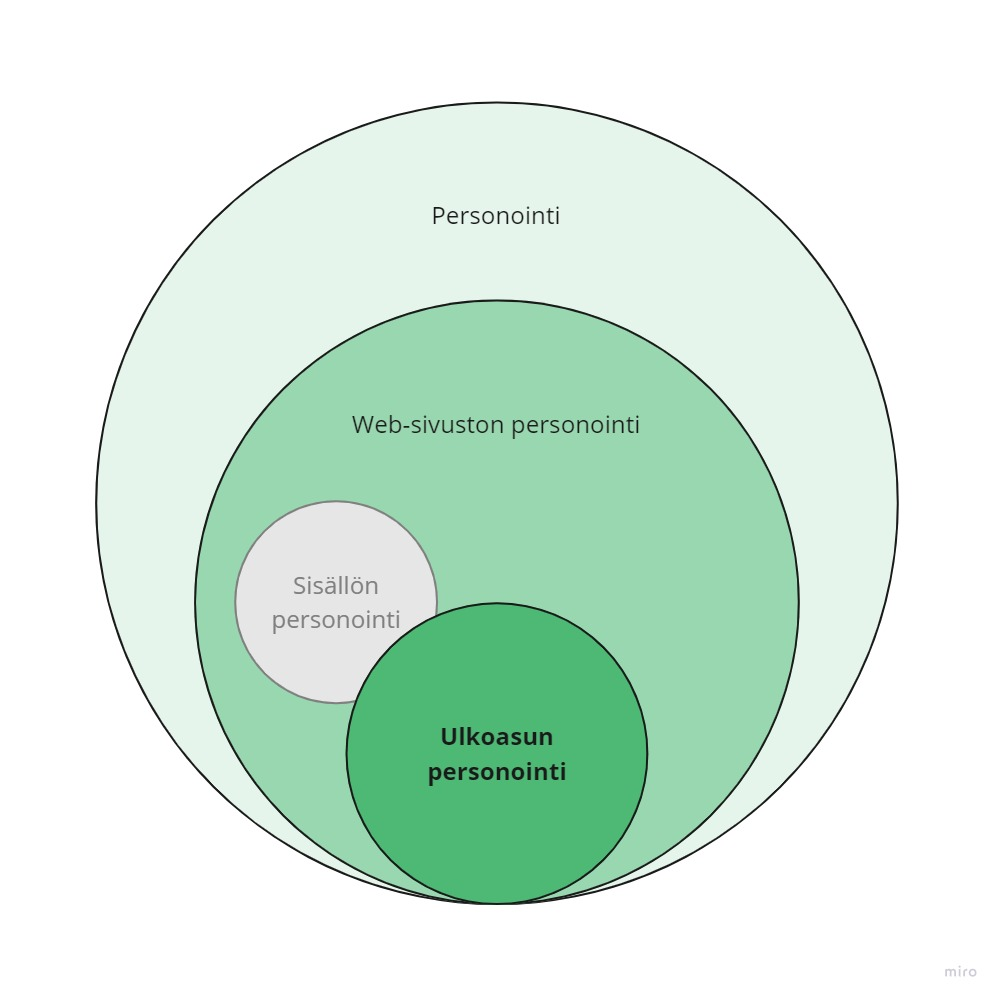
\includegraphics[width=0.6\textwidth]{images/thesis-scope.jpg}
    \caption{Työssä tarkastellaan web-sivuston ulkoasun personointia. Sisällön
    personointi on rajattu työn ulkopuolelle.~\label{fig:thesis-scope}}
\end{figure}

Vaikka web-sivustojen personointia on tutkittu verrattain pitkään, käytännön
hyödyntäminen toimialalla on vielä harvinaista. Sivuston ulkoasu suunnitellaan
nykyäänkin lähtökohtaisesti ihmisen toimesta, ja myös ulkoasusuunnitelman
tulkitseminen ja ohjelmoiminen lopulliseksi sivustoksi on manuaalista työtä.
Käyttäjille tai edes käyttäjäryhmille ei siis ole kustannustehokasta suunnitella
personoituja versioita sivustoista. Yhden ja saman version jakelu kaikille
sivuston käyttäjille ei kuitenkaan ole aina optimaalista, sillä käyttäjillä on
eri mieltymyksiä muun muassa kulttuuritaustasta ja iästä
riippuen~\cite{10.1145/2556288.2557052}.

Selvitän työssäni, mitä menetelmiä web-sivuston ulkoasun eri osa-alueiden
personointiin on olemassa. Tarkasteltavia osa-alueita ovat sivuston asettelu,
värit, typografia sekä kuvat. Tarkastelen työssä myös eri personointimenetelmien
toimintatapoja. Monet tarkasteltavista menetelmistä perustuvat matemaattisen
optimointiin, mutta hyödyntävät tuloksissaan lisäksi käyttöliittymäsuunnittelun
heuristiikkoja, kuten tekstin luettavuuskriteerejä. Sivuston eri osa-alueiden
personointia ja personointimenetelmien toimintatapoja tarkastellaan
luvussa~\ref{personalization}.

Vertailen työssä myös personointimenetelmien käyttöönoton vaivattomuutta ja
niillä saavutettavaa hyötyä. Pyrin vertailun avulla löytämään
personointimenetelmät, joista saa suurimman hyödyn pienimmällä vaivalla.
Pisteytyskriteeristö ja vertailun tulokset on esitelty
luvussa~\ref{personalization-comparison}.

\clearpage
\section{Tausta}\label{background}

Web-ohjelmistokehitys on muuhun ohjelmistokehitykseen verrattuna nuori ala ja
edelleen jatkuvassa murroksessa. Tässä luvussa selvitetään web-suunnittelun ja
-kehityksen nykytilannetta työn taustatiedoksi. Luvussa käsitellään myös
personoinnin kannalta oleellinen web-analytiikan ala (engl.~\textit{web
analytics}) ja tarkastellaan yleisesti käyttöliittymän tuottamista
laskennallisesti.

\subsection{Web-sivuston ulkoasun toteutus}

Ulkoasun toteutus jakaantuu kahteen selkeään vaiheeseen. Suunnittelija tuottaa
sivuston ulkoasusta suunnitelman, jonka pohjalta kehittäjä tuottaa lopullisen
sivuston. Nämä kaksi vaihetta käsitellään tässä luvussa. Esimerkinomainen
havainnollistus web-sivuston ulkoasun toteutuksesta on esitetty
kuvassa~\ref{fig:website-implementation}.

\subsubsection{Ulkoasun suunnittelu}\label{background-web-design}

Web-suunnittelu (engl.~\textit{web design}) on käytännön tasolla lähellä muita
graafisen suunnittelun aloja kuten printtisuunnittelua, vaikka mediana web
tarjoaa paljon enemmän mahdollisuuksia vuorovaikutukseen. Web-suunnittelun
päätuotos eli ulkoasusuunnitelma (engl.~\textit{layout}) on ei-vuorovaikutteinen
vektorikuva siitä, miltä toteutettavan sivuston tulee näyttää.
Ei-vuorovaikutteisesta luonteestaan huolimatta ulkoasusuunnitelma ei nykyään ole
enää pelkkä rasterikuva (engl.~\textit{raster image}), toisin kuin yleisesti
vielä 2000-luvulla. Vuonna 2010 julkaistun Sketch-ohjelmiston myötä
vektorimuotoisesta ulkoasusuunnittelusta on tullut
valtavirtaa~\cite{webdesignmuseum_2022}, ja Sketchin rinnalle on viime
vuosikymmenellä noussut myös muita vektoripohjaisia suunnitteluohjelmistoja,
kuten Adobe XD ja Figma. Ulkoasusuunnitelman lisäksi suunnittelija tuottaa usein
osittain interaktiivisia prototyyppejä, joilla sivuston toimintaa voi esitellä
ulkoasusuunnitelman kautta esimerkiksi asiakkaalle ennen toteutusta.
Ulkoasusuunnitelmaan tehdään tarvittavat mukautukset eri käyttäjäryhmille vain
ennalta sovittujen määrittelyjen ja palvelumuotoilun (engl.~\textit{service
design}) pohjalta. Yleisin tällainen mukautus on oman ulkoasusuunnitelman
tuottaminen eri laitetyypeille, kuten mobiili-, tabletti- ja työpöytälaitteille.
Laitetyyppeihin perustuvaa mukauttamista kutsutaan responsiiviseksi
web-suunnitteluksi (engl.~\textit{responsive web design}), josta kerrotaan lisää
luvussa~\ref{responsive-web-design}. Yksilötason personointia
ulkoasusuunnitelmiin ei yleensä sisällytetä.

\subsubsection{Ulkoasun kehitys}\label{background-web-development}

Ulkoasun kehittäjän (engl.~\textit{front-end developer}) tehtävä on kääntää
ulkoasusuunnitelma toimivaksi sivustoksi. Vektorimuotoiseen ulkoasusuunnitelmaan
on upotettu kaikki kehittäjän tarvitsemat yksityiskohdat ulkoasun
toteuttamiseen, kuten kirjasintyyppi ja -koko, marginaalit ja värikoodit.
Kehittäjä hyödyntää ulkoasusuunnitelman käsittelyyn joko samoja työkaluja kuin
suunnittelija tai varta vasten ulkoasusuunnitelmien käsittelyyn tarkoitettuja
kehittäjätyökaluja, kuten Zeplin-ohjelmistoa.

Karkeasti yleistäen web-sivuston ulkoasun kehityksessä on pääosassa kolme
teknologiaa: HTML-merkintäkieli (\textit{HyperText Markup Language}),
CSS-säännöstö (\textit{Cascading Style Sheets}) ja JavaScript-ohjelmointikieli.
HTML-merkintäkielen avulla määritetään sivuston rakenne ja sen eri osien
rakenteellinen merkitys. Selain ymmärtää HTML-rakenteen eri osien merkityksen ja
pystyy piirtämään ne sivulle oikealla tavalla. CSS-säännöstön avulla määritetään
sivuston osien tyyli ja asettelu, eli se on HTML-rakenteen lisäksi merkittävässä
osassa ulkoasusuunnitelmaa toteuttaessa. JavaScript on ainoa web-alustalla
kattavasti tuettu varsinainen ohjelmointikieli. Sillä on mahdollista luoda
vuorovaikutusta käyttäjän ja sivuston välille.

Nykyään kehittäjä rakentaa sivuston ulkoasua harvemmin enää pelkästään näillä
kolmella perusteknologialla. Niiden päälle on kehitetty teknologioita ja
kirjastoja, jotka vähentävät toistuvaa työtä ja huolehtivat osaltaan hyvistä
käytänteistä, kuten saavutettavuudesta. Nämä teknologiat hyödyntävät enenevissä
määrin JavaScript-ohjelmointikieltä, mikä on tuonut sivuston ulkoasun kehitystä
lähemmäs perinteisempää ohjelmistokehitystä. Aiemmin sivustoja oli yleistä
rakentaa lähes ilman ohjelmointityötä pelkän HTML-merkintäkielen ja
CSS-tyylisäännöstön avulla. Sivustojen käytettävyyttä parannettiin kevyen
JavaScript-skriptauksen avulla siellä ja täällä, mutta varsinainen
ohjelmointityö rajoittui yleensä palvelinpuolelle. Palvelinpuolen kehitystä ei
käsitellä tässä työssä työn rajauksesta johtuen.

Sittemmin tärkeä edistysaskel sivuston ulkoasun kehityksessä on tapahtunut
2010-luvun loppupuolella, kun JavaScript-käyttöliittymäkirjastot, kuten React ja
Vue, ovat yleistyneet merkittävästi. Käyttöliittymäkirjastojen myötä ulkoasu
rakennettaan toisistaan riippumattomilla web-komponenteilla. Yksittäinen
komponentti toteuttaa jonkin rajatun ja selkeän toiminnallisuuden, ja
komponentteja on helppo uudelleenkäyttää myöhemmin. Komponentit myös
mahdollistavat osaltaan suunnittelujärjestelmien (engl.~\textit{design system})
luomisen jo projektin alussa. Suunnittelujärjestelmä sisältää yleensä projektin
komponenttikirjaston, joka käsittää sivuston rakennuspalikat, kuten lomake- ja
tekstielementit. Komponenttien kehityksessä käytetään kuitenkin yhä samaa
perusteknologiaa kuin aiemminkin, eli HTML-merkintäkieltä, CSS-tyylisäännöstöä
ja JavaScript-ohjelmointikieltä.

\begin{figure}[h]
    \centering
    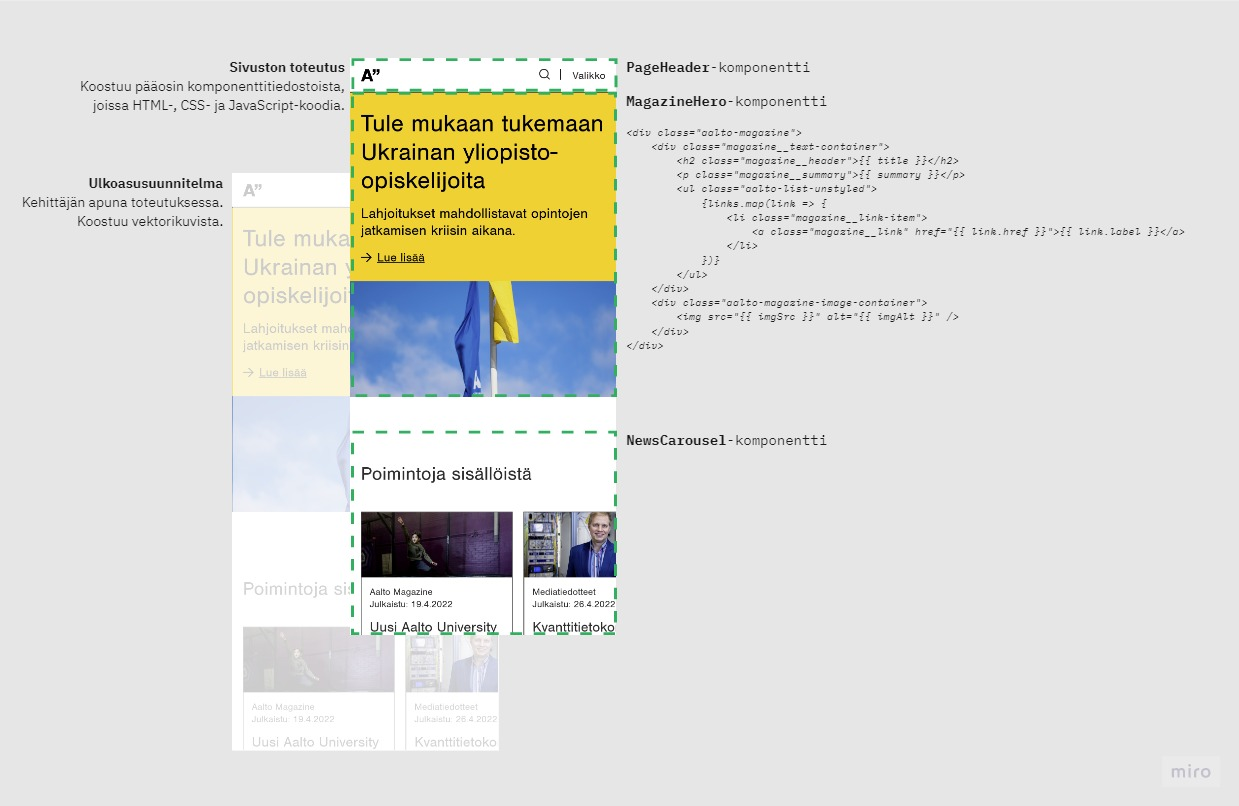
\includegraphics[width=\textwidth]{images/website-implementation.jpg}
    \caption{Yksinkertaistettu ja kuvitteellinen havainnollistus web-sivuston~\cite{aalto-website}
    toteutuksesta. MagazineHero-komponentin yhteydessä on esitetty komponentin
    esimerkinomainen HTML-rakenne.~\label{fig:website-implementation}}
\end{figure}

\subsection{Web-analytiikka}

Personointi on käyttäjästä kerätyn tiedon pohjalta tehtävää automaattista
mukauttamista. Web-analytiikka on siksi tärkeässä osassa personoinnissa, sillä
tarvittava tieto käyttäjästä kerätään yleensä analytiikan avulla. Burby
ym.~\cite{burby2007web} määrittelevät web-analytiikan olevan käyttötiedon
keräämisen, analyysin ja raportoinnin pohjalta tehtävää web-sivuston
optimointia. He jakavat kerättävän tiedon kolmeen eri luokkaan. Ensinnäkin osa
tiedosta on määrämuotoista, kuten kävijöiden määrä sivustolla tai vuoden myynti
euroissa. Toinen osa tiedosta on suhdelukumuotoista, esimerkiksi sivukatseluiden
määrä per kävijä. Kolmannen osan kerättävästä tiedosta muodostavat keskeiset
suorituskykyindikaattorit (engl.~\textit{Key Performance Indicator, KPI}), jotka
ovat usein yhdistelmä suhdeluku- ja määrämuotoista tietoa.

Burby ym.~luokittelevat kerättävän tiedon kolmeen tasoon tarkkuuden perusteella.
Yleisintä on koottu eli aggregoitu tieto, esimerkiksi kävijöiden määrä
etusivulla koko sivuston olemassaolon ajalta. Segmentoitu tieto on jokin
tarkempi näkökulma koottuun tietoon nähden, esimerkiksi kävijöiden määrä
sijainnin, kuten maan tai kaupungin, perusteella. Web-analytiikka mahdollistaa
myös yksittäisen kävijän seuraamisen. Yksilötason tiedoista näkee esimerkiksi
millä sivustoilla yksittäinen kävijä on sivustovierailunsa aikana käynyt.

Teknisesti web-analytiikassa hyödynnettävää tietoa voi kerätä muutamalla eri
tavalla. Zheng ja Peltsverger~\cite{zheng2015web} luokittelevat neljä eri tasoa
web-käyttötiedon keräämiseen. Tietoliikenteen tasolla voidaan kerätä liikenteen
reititykseen käytettäviä tietoja, kuten käyttäjän IP-osoite. IP-osoitteen avulla
on muun muassa mahdollista arvioida karkeasti käyttäjän sijainti. Selaimen ja
palvelimen väliseen kommunikointiin käytettävän hypertekstin siirtoprotokollan
(engl.~\textit{HyperText Transfer Protocol, HTTP}) pyyntö- ja vastaussanomista
voidaan kerätä metatietoa selailusta, esimerkiksi tieto siitä millä sivuilla
käyttäjä on vieraillut. Sovellustasolla, eli palvelimella tai selaimessa,
voidaan kerätä tietoa sivuston käytöstä, esimerkiksi mitä tietoja käyttäjä on
lähettänyt jonkin lomakkeen kautta. Kerättyä tietoa voidaan yhdistää ulkoisista
lähteistä, kuten sähköpostikampanjoista, kerättyyn tietoon.

Tämä Zhengin ja Peltsvergerin määrittämä neljäs taso, eli ulkoisista lähteistä
kerätty tieto, voi olla ongelmallista tietosuojan kannalta. Yleinen keino
seurata käyttäjää ulkoisilla sivustoilla on asettaa yksilöivä eväste, eli pieni
tekstitiedosto, käyttäjän laitteelle. Tämän jälkeen ulkoiset sivustot, jotka
ottavat yhteyttä lähdesivustoon, välittävät samalla lähdesivustolle sen
käyttäjän laitteelle asettamat evästeet. Tällöin lähdesivusto pystyy
tunnistamaan käyttäjän ja hyödyntämään uutta tietoa tämän ulkoisesta
web-selailusta analytiikassaan. Nämä niin kutsutut kolmannen osapuolen evästeet
ovat lähitulevaisuudessa poistumassa käytöstä ilmeisten tietosuojariskien
takia~\cite{third-party-cookies-phaseout}, millä voi olla arvaamattomia
vaikutuksia web-analytiikan ja -liiketoiminnan kannalta.

\subsection{Käyttöliittymän tuottaminen laskennallisesti}

Ennen tarkempaa personoinnin tarkastelua esitellään vielä tutkimusta liittyen
käyttöliittymän laskennalliseen tuottamiseen, mikä on oleellista taustatietoa
varsinkin sivuston asettelun personoinnin kannalta. Käyttöliittymän
laskennallinen tuottaminen laajentaa luvussa~\ref{background-web-design}
kuvattua web-suunnitteluprosessia, sillä nämä laskennalliset menetelmät toimivat
apuna varsinkin suunnitteluvaiheessa. Laskennallisen menetelmän avulla
suunnittelija voi saada välitöntä palautetta ulkoasusuunnitelman laadusta
menetelmän määrittämiin kriteereihin perustuen. Menetelmä voi myös suoraan
suositella vaihtoehtoisia ulkoasusuunnitelmia.

Oulasvirta ym.~\cite{9000519} esittelevät menetelmiä käyttöliittymien
laskennalliseen tuottamiseen ja kohentamiseen. He tarkastelevat aihetta
kombinatorisen optimoinnin (engl.~\textit{combinatorial optimization})
näkökulmasta. Kombinatorinen optimointi tarkoittaa optimaalisen tuloksen
löytämistä diskreetistä ja äärellisestä joukosta tuloksia. Kombinatoriseen
optimointiin liittyy vahvasti kokonaislukuohjelmointi (engl.~\textit{integer
programming}). Kokonaislukuohjelmoinnissa olennaista on se, että optimoitavat
muuttujat ovat nimenmukaisesti kokonaislukuja, mikä poistaa tarpeen esimerkiksi
liukulukujen huomioimiselle ohjelmakoodissa. Kokonaislukuohjelmoinnin käyttö on
järkevää silloin, kun optimoitava suure on kokonaisluku, kuten esimerkiksi
sarakkeiden määrä ulkoasusuunnitelmassa.

Oulasvirta ym.~näyttävät, että kombinatorinen optimointi on keino esittää
matemaattisena ongelmana ulkoasusuunnittelun heuristiikat ja suunnittelun aikana
tehtävät päätökset, kuten elementtien keskinäinen koko ja järjestys. He
tähdentävät myös, että kombinatorinen optimointi ei tarvitse erillistä
opetusdataa, kuten menetelmät, jotka hyödyntävät ohjattua koneoppimista
(engl.~\textit{supervised machine learning}). He nostavat esille laskennallisen
käyttöliittymäsuunnittelun hyötyinä muun muassa kohonneen laadun ja
johdonmukaisuuden, kyvyn tukea suunnittelijaa erityisesti hankalissa
erikoistapauksissa ja lisääntyneen ymmärryksen ihmisen ja tietokoneen välisestä
vuorovaikutuksesta suunnittelijoiden keskuudessa.

Käyttöliittymän laskennalliseen tuottamiseen palataan
luvussa~\ref{layout-personalization}, jossa tarkastellaan sivuston asettelun
personointimenetelmiä.

\clearpage
\section{Personointi}\label{personalization}

Käytän työssäni Blomin~\cite{10.1145/633292.633483} vuonna 2000 julkaisemaa
personoinnin taksonomiaa. Sen mukaan personoinnilla tarkoitetaan järjestelmän
muuttamista tavalla, jossa sen henkilökohtainen merkitys käyttäjän näkökulmasta
kasvaa. Tämä personoinnin prosessi on esitetty kuvassa~\ref{fig:personalization}.
Personoinnin myötä tehdyt muutokset ovat lähtökohtaisesti käyttäjälle pysyviä,
joskin ne voivat muuttua edelleen käytön jatkuessa. Personoinnin perusteeksi
kerätty tieto voi olla hyvin erilaisista lähteistä, kuten asiointihistoriasta,
julkishallinnon rekistereistä tai web-sivuston tapauksessa sivuston
web-analytiikasta ja lokitiedoista. Tieto, jonka pohjalta personointia tehdään
voi olla myös käyttäjän itse ilmoittamaa, joskin tällöin puhutaan yleensä
kustomoinnista. Personointia voidaan tehdä missä tahansa rajapinnassa, jossa on
käyttäjän ja palvelun välistä vuorovaikutusta, kuten toimipiste-, puhelin- tai
web-asioinnissa. Työni keskittyy web-asioinnin personointiin ja nimenomaan
web-sivuston ulkoasun personointiin.

\begin{figure}[h]
    \centering
    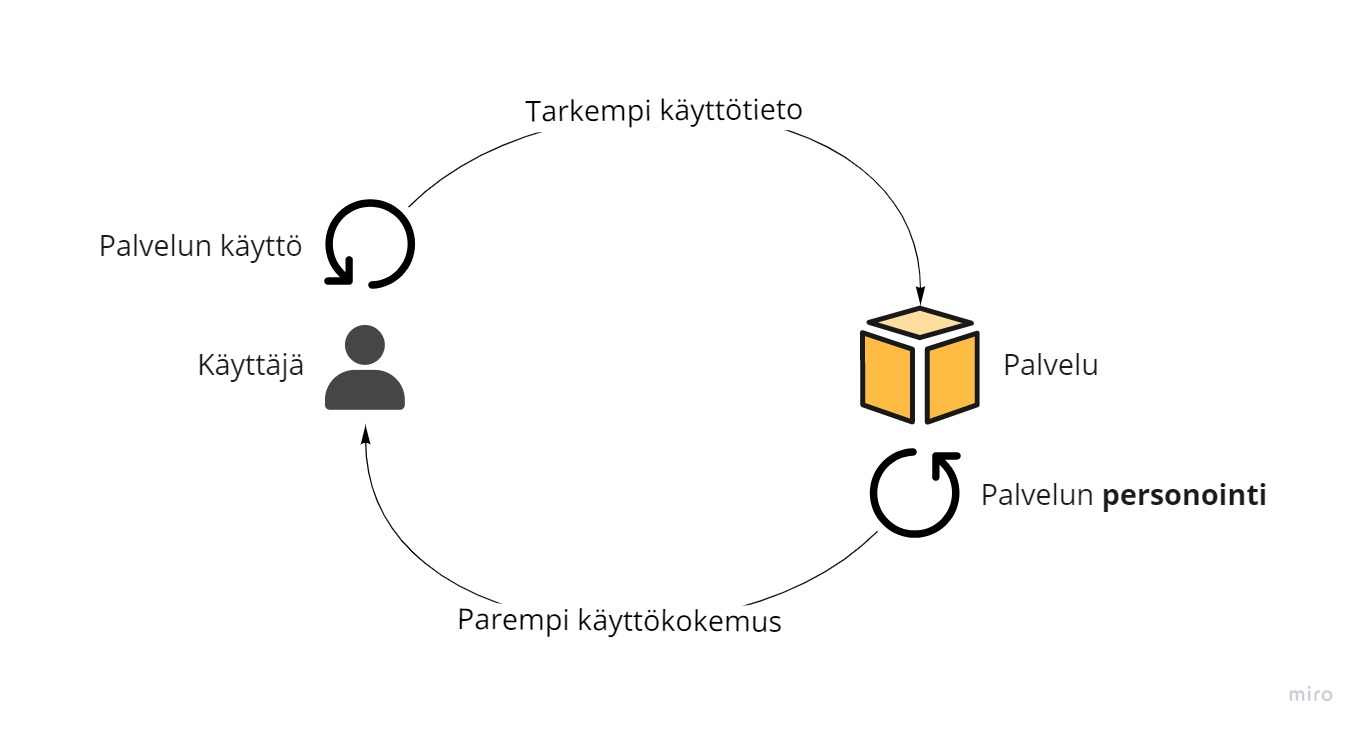
\includegraphics[width=\textwidth]{images/personalization.jpg}
    \caption{Käyttökokemusta voidaan parantaa personoimalla palvelua esimerkiksi
    web-analytiikan avulla kerätyn käyttötiedon
    perusteella.~\label{fig:personalization}}
\end{figure}

Ennen kuin personoinnin näkökulmia ja varsinaisia menetelmiä käydään läpi, on
tärkeää tarkentaa, miksi personointia ylipäätään kannattaa hyödyntää
sivustolla.

\subsection{Personoinnin hyödyt}\label{personalization-pros}

Tarve personoinnille vaihtelee sivuston mukaan, mutta Blomin taksonomian
mukaisesti tarpeet voidaan jakaa karkeasti kahteen luokkaan. Ensimmäinen luokka
käsittää ohjelmiston, kuten sivuston, kanssa työskentelyyn liittyvät tarpeet,
jotka voidaan jakaa kolmeen ryhmään. Ensinnäkin personointi mahdollistaa
tehokkaamman pääsyn käyttäjälle tärkeään sisältöön. Blom mainitsee esimerkkinä
kirjanmerkkien käytön sivustolla, mutta nykyaikaisempi esimerkki voisi olla
suosittelualgoritmin automaattisesti korostamat sisällöt. Toisekseen
personoinnilla on mahdollista optimoida prosesseja, kuten lomakkeen täyttöä
sivustolla. Osa lomakkeen vaiheista voidaan ohittaa, jos tiedot saadaan haettua
suoraan taustajärjestelmistä. Kolmanneksi personoinnilla voidaan huomioida
yksilölliset erot, kuten näkövammat ja liikunnalliset rajoitteet. Esimerkiksi
näkövammaisille voidaan tarjota suurempikontrastinen versio sivustosta.
Yksilölliset erot ja rajoitteet voivat olla lähtöisiä myös käyttöympäristöstä,
kuten esimerkiksi kirkas auringonvalo tai äänekäs taustahäly. Myös
tämäntyyppisten rajoitteiden kaipaamaa personointia käsitellään osana tätä
työtä.

Toinen Blomin taksonomian mukainen luokka käsittää sosiaaliset tarpeet, jotka
voidaan jakaa kahteen ryhmään. Ensimmäisenä Blom mainitsee ihmisen tarpeen
herättää tietynlainen tunnereaktio myös vuorovaikutuksessa ohjelmiston kanssa.
Blom pohtii, että samaan tapaan kuin ihmisellä on tapana sisustaa työtilaansa,
sama personoinnin tarve koskee myös ihmisen käyttämiä ohjelmistoja. Toisena Blom
mainitsee ihmisen tarpeen ilmaista omaa identiteettiään, jota hän tarkentaa
vielä ihmisen tarpeella liittää itsensä johonkin yhteisöön. Nämä tarpeet
mielessä pitäen henkilö voidaan saada kokemaan itsensä enemmän tervetulleeksi
personoidulla sivustolla.

Vesanen~\cite{10.1108/03090560710737534} pohtii laajemmin personoinnin
määritelmää erityisesti palveluntarjoajan näkökulmasta. Yleisesti voidaan
todeta, että personoinnin tavoitteena on ohjata käyttäjän toimintaa sivuston
palveluntarjoajan tavoitteiden mukaisesti ja yleensä nimenomaan joko lisätä
palveluntarjoajan tuloja tai vähentää sen menoja. Esimerkiksi verkkokauppa voi
lisätä myyntiä personoimalla asiakkaalle suositeltavia tuotteita tämän
ostohistorian perusteella. Sitä vastoin kunta voisi asiointisivustoaan
personoimalla nostaa vierailijalle ajankohtaiset lomakkeet heti etusivun alkuun
ja täten lisätä verkkoasiointia ja vähentää kalliimpaa puhelinasiointia. Blomin
ja Vesasen esittämät personoinnin hyödyt on kiteytetty ja yhdistetty
kuvaan~\ref{fig:personalization-benefits}.

\begin{figure}[h]
    \centering
    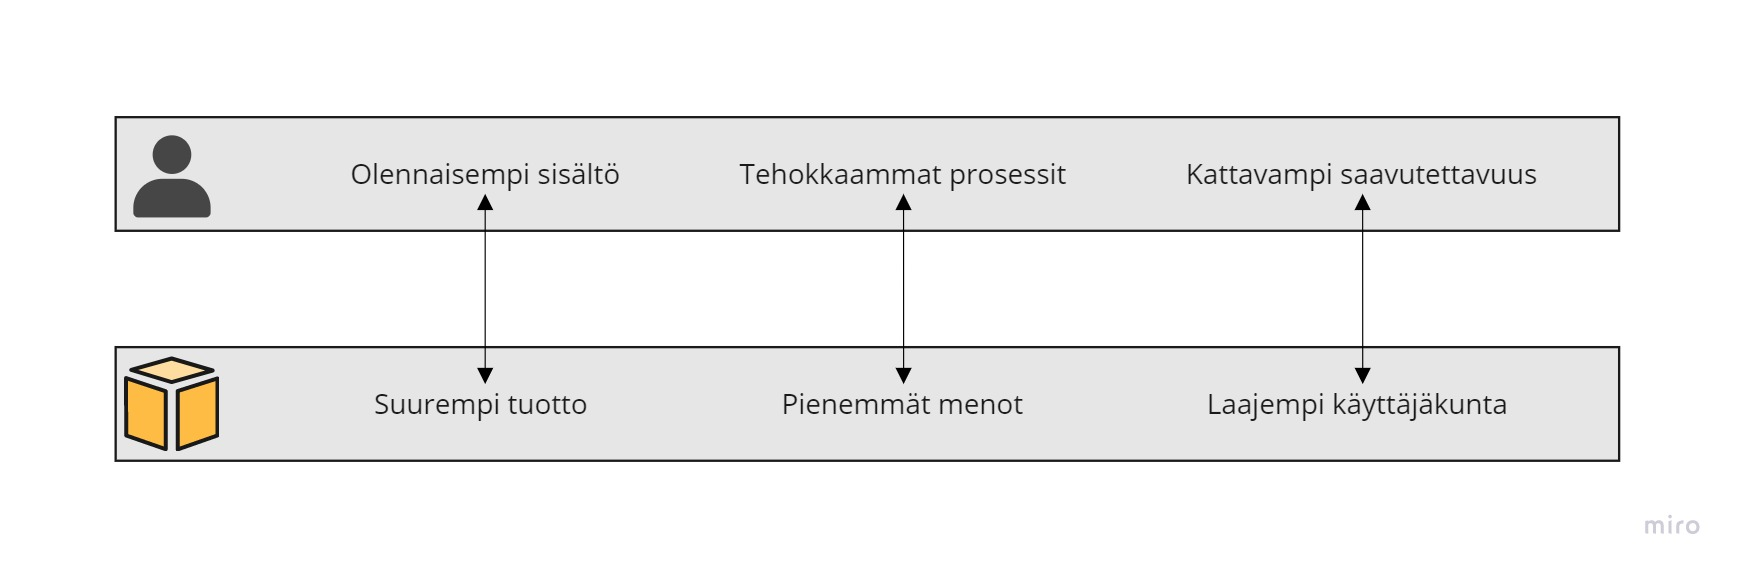
\includegraphics[width=\textwidth]{images/personalization-benefits.jpg}
    \caption{Personoinnin hyödyt karkealla tasolla käyttäjän ja
    palveluntarjoajan näkökulmasta.~\label{fig:personalization-benefits}}
\end{figure}

Personoinnista on hyötyä myös yhteiskunnallisella tasolla. Personointi
mahdollistaa yksilöllisen tiedonvälityksen kokoluokassa, joka ei aiemmin ole
ollut mahdollinen. Painettu media skaalautuu hyvin, ja sen kautta tietoa on
ollut mahdollista levittää laajalle jo vuosisatoja, mutta sen personointi on
liki mahdotonta tai ainakin erittäin kallista. Toinen ääripää, eli tiedonvälitys
henkilöltä toiselle, on aina personoitua, mutta ei mahdollista tehokasta
tiedonvälitystä suurille väkijoukoille. Julkinen valta ja muut yleishyödylliset
toimijat voivat siis hyödyntää personointia tiedonvälityksessä tavoittaakseen
suurempia yleisöjä. Tästä on ollut hyötyä esimerkiksi koronaviruspandemian
aikana, kun rokotekampanjoiden verkkoviestintää on voitu personoida tärkeille
yleisöille~\cite{sanchez_2022}.

Personoidulla tiedonvälityksellä on kuitenkin myös kääntöpuolensa, jota
tarkastellaan seuraavaksi osana personoinnin haittoja.

\subsection{Personoinnin haitat}\label{personalization-cons}

Personoinnissa on hyötyjen lisäksi selkeitä kipukohtia. Personointi perustuu
käyttäjästä kerättyyn tietoon. Tietoa kerätään mahdollisesti monesta eri
kanavasta, ja on tärkeää, että tietojen keräämiseen on aina käyttäjän suostumus.
Tietolähteiden lisääntyessä käyttäjä ei välttämättä enää ole selvillä siitä,
mitä tietoa on suostunut luovuttamaan ja mihin. Fernandez
ym.~\cite{10.1145/3476087} löysivät, että Euroopan Unionin yleisen
tietosuoja-asetuksen (engl. \textit{General Data Protection Regulation, GDPR})
myötä yleistyneet evästesuostumuslomakkeet ohitetaan usein lukematta.
Suostumusta kysytään lähes jokaisella sivustolla, koska web-analytiikka ja
kohdennettu mainonta on niin yleistä. Asenteet sisällön personoinnin osalta ovat
muuttuneet kielteisempään suuntaan, kun vielä 90-luvulla sisällön personointi
nähtiin verkkoon siirtyvän printtimedian pelastajana~\cite{adams_1995}.

Arkielämän teknistyessä käyttäjälle ei myöskään ole välttämättä aina selvää,
minkälaista tietoa hänestä on edes mahdollista kerätä. Tiedot kuten hiiren
liike, näppäimistösyöte, laitetiedot ja jossain määrin myös selailuhistoria ovat
web-analytiikan käytettävissä. Laitetietojen pohjalta käyttäjästä voi muodostaa
tunnisteen, jota on käytännössä mahdoton muuttaa tai pyyhkiä pois vaihtamatta
laitetta. Evästeiden avulla isot mainosverkostot pystyvät seuraamaan käyttäjää
sivustolta toiselle ja personoimaan mainontaa selailukäyttäytymisen perusteella.

Personointi ei aina ole toivottua. Monet alustapohjaiset teknologiayritykset
ovat viime vuosina panostaneet erilaisiin suosittelualgoritmeihin kohdentaakseen
sisältöään paremmin. Suosittelualgoritmit toimivat hyvin suurelle osalle
käyttäjäkunnasta, mutta saattavat hankaloittaa palvelun käyttöä pienelle osalle,
johon kuuluvat eivät sovi hyvin algoritmin luokitteluun. Suosittelualgoritmit
ovat myös korvanneet palveluiden aiemmin käyttäjälle tarjoamia
kustomointimahdollisuuksia, kuten sisällön järjestelyasetuksia, mikä on
hankaloittanut palveluiden käyttöä~\cite{patel_2022}.

Luvussa~\ref{personalization-pros} kuvattu tiedonvälityksen personointi voi olla
myös haitaksi. Jos hyväntahtoiset toimijat, kuten terveysvirastot, pystyvät
personoimaan tiedonvälitystä avainryhmille, sama onnistuu myös pahantahtoisilta
toimijoilta. Tiedonvälityksen personointi voi muodostua ongelmaksi myös
itsestään. Spohr~\cite{doi:10.1177/0266382117722446} näyttää, että sisällön
personointi sosiaalisen median alustoilla johtaa sisällön yksipuolistumiseen,
vähentäen näin käyttäjän altistumista erilaisille näkökulmille.

Tämän työn aihe eli sivuston ulkoasun personointi on kuitenkin verrattain
harmiton personoinnin osa-alue. Sen haittapuolena on lähinnä lisääntynyt
sivuston tekninen monimutkaisuus käytetystä menetelmästä riippuen.

\subsection{Näkökulmat ulkoasun personointiin}\label{personalization-aspects}

Web-sivuston ulkoasun personointia tarkastellaan työssäni käyttäjälähtöisistä ja
ympäristölähtöisistä näkökulmista.

Osa käyttäjälähtöisistä näkökulmista perustuu käyttäjän fyysisiin
ominaisuuksiin. Käyttäjällä voi olla esimerkiksi näkö- ja liikuntarajoitteita,
jotka vaikuttavat merkittävästi sivuston käyttöön. Muita fyysisiä ominaisuuksia,
joiden näkökulmasta personointia tarkastellaan, ovat ikä ja sukupuoli. Fyysisten
ominaisuuksien lisäksi myös kulttuuritausta ja kieli, koulutustaso,
kiinnostuksen kohteet ja asiointihistoria, sosiaaliset verkostot ja mieliala
ovat ominaisuuksia, joiden näkökulmasta sivuston ulkoasun personointia
tarkastellaan.

Ympäristölähtöiset näkökulmat liittyvät sivuston selailuun käytettävän laitteen
ominaisuuksiin ja toisaalta myös laajemmin käyttöympäristön ominaisuuksiin.
Laitteen ominaisuuksia, joiden näkökulmasta personointia tarkastellaan, ovat
laitteen näyttökoko ja suorituskyky. Laajemmin käyttöympäristöön liittyviä
personoinnin näkökulmia ovat verkkoyhteyden nopeus, sijainti sekä vuoden- ja
kellonaika. Laitteen antureita voidaan hyödyntää lähiympäristön havainnoimiseen,
jolloin personoinnissa voidaan hyödyntää ympäristön kirkkautta, lämpötilaa,
taustamelun äänenvoimakkuutta sekä liikeominaisuuksia, kuten tärinää ja
nopeutta.

Näitä näkökulmia tarkastellaan erityisesti
luvussa~\ref{personalization-comparison}. Seuraavissa alaluvuissa esitellään
personoinnin menetelmiä sivuston eri osa-alueiden näkökulmasta. Tarkasteltavat
sivuston osa-alueet on esitetty kuvassa~\ref{fig:website-areas}.

\begin{figure}[h]
    \centering
    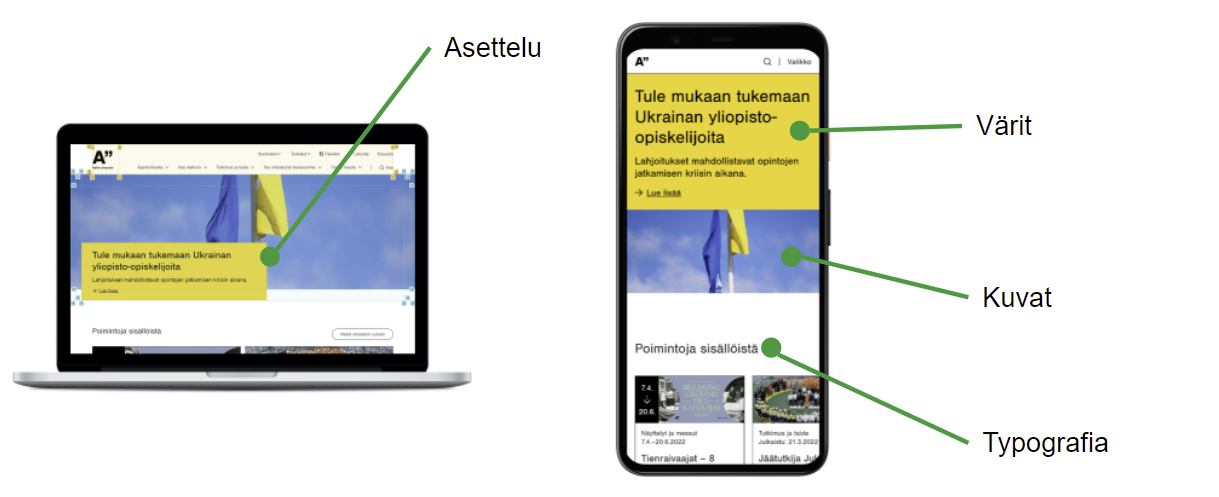
\includegraphics[width=\textwidth]{images/website-areas.png}
    \caption{Personoinnin näkökulmia tarkastellaan työssä neljän eri sivuston
    osa-alueen kautta: asettelu, värit, typografia ja kuvat. Kuvissa
    Aalto-yliopiston etusivu~\cite{aalto-website}.~\label{fig:website-areas}}
\end{figure}

\subsection{Asettelun personointi}\label{layout-personalization}

Sivun asettelu määrittää sivuston perusrakenteen ja sivun sisällön keskinäisen
järjestyksen. Tyypillisesti sivuston yksittäisellä sivulla on vähintään
ylätunniste (engl.~\textit{header}), sisältöalue (engl.~\textit{content area})
ja alatunniste (engl.~\textit{footer}). Ylätunniste ja alatunniste pysyvät
yleensä suurin piirtein muuttumattomina sivustolla navigoidessa, mutta
sisältöalueen sisältö luonnollisesti vaihtuu sivun mukaan. Ylätunniste ja
alatunniste ovat valikonomaisia sivuston osia. Ylätunniste sijaitsee aina sivun
alussa ja alatunniste sivun lopussa. Niiden asettelun personointi ei ole
mielekästä, joten niitä ei tarkastella enempää tässä alaluvussa.

Sivun asettelun lisäksi myös valikoiden asettelua on mahdollista personoida.
Valikoiden asettelu eroaa normaalista sisällöstä hivenen siksi, että valikon
vaihtoehdoilla on vähemmän vapausasteita verrattuna sisällön asetteluun.
Vaihtoehtojen järjestys voi muuttua, niitä voidaan piilottaa ja niitä voidaan
korostaa esimerkiksi lihavoinnilla. Ne eivät siis esimerkiksi voi
lähtökohtaisesti siirtyä valikon ulkopuolelle. Valikoiden asettelun personointia
tarkastellaan tarkemmin luvussa~\ref{menu-personalization}.

Sisältöalueen asettelu perustuu nykyään lähtökohtaisesti ruudukkorakenteeseen
(engl.~\textit{grid layout}). Ruudukkorakennetta on havainnollistettu
kuvassa~\ref{fig:grid-layout}. Ruudukko koostuu sivustosta ja päätelaitteen
näyttökoosta riippuen yleensä n.~1--16 sarakkeesta (engl.~\textit{column}),
jotka on erotettu toisistaan vakiosuuruisella marginaalilla
(engl.~\textit{margin}). Sarakkeiden leveys, joka on kääntäen verrannollinen
sarakkeiden määrään, perustuu suhteelliseen osaan saatavilla olevasta
ruudukkoalueen (engl.~\textit{grid container}) leveydestä, ja sarakkeiden leveys
muuttuu yhdessä ruudukkoalueen kanssa. Ruudukkoalueelle sijoittuvat elementit
(engl.~\textit{element}), kuten tekstipalstat ja kuvat, voivat kattaa yhden tai
useamman sarakkeen leveyden. Elementtien leveys määritetään kuitenkin nimenomaan
sarakkeiden kautta, eivätkä ne voi vapaasti laajentua leveyssuunnassa niiden
sisällön kasvaessa. Sen sijaan elementit laajenevat tarvittaessa
pituussuunnassa. Tyypillisesti sivustot eivät mahdukaan kokonaan kerralla
näytölle, vaan niitä pitää vierittää alaspäin jolloin lisää sisältöä tulee
näkyville.

\begin{figure}[h]
    \centering
    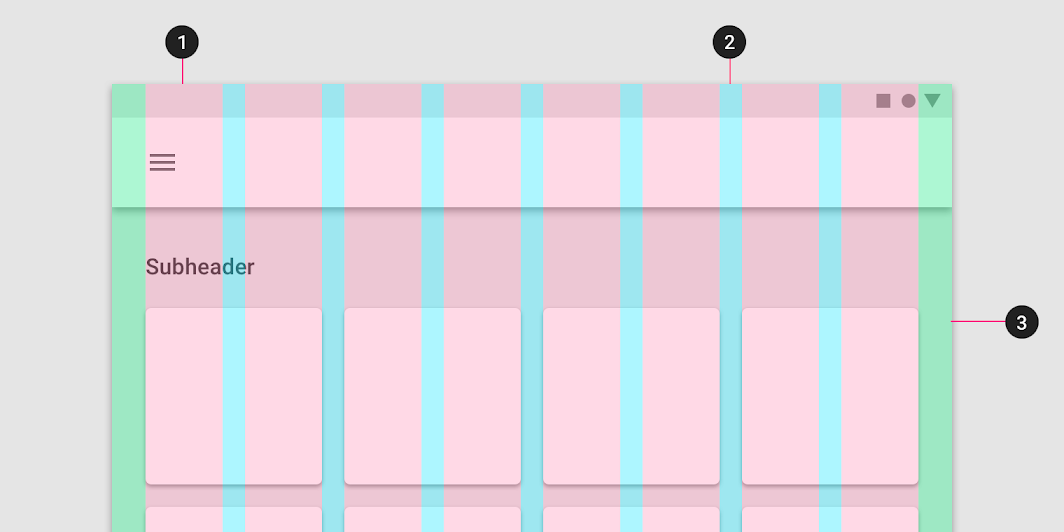
\includegraphics[width=\textwidth]{images/grid-layout.png}
    \caption{Ruudukkorakenne koostuu sarakkeista (1), jotka on erotettu
    marginaaleilla (2) toisistaan. Ruudukkoalueella voi myös olla
    marginaalit, joilla se erotetaan sivun reunoista ja keskitetään sivulle
    (3).~\cite{material-design-grid}~\label{fig:grid-layout}}
\end{figure}

\subsubsection{Responsiivinen web-suunnittelu}\label{responsive-web-design}

Ennen 2010-lukua asettelu tehtiin lähtökohtaisesti staattisesti, tarkoittaen
että sivun sisältöalueella oli ennalta määrätty leveys. Leveys oli yleensä
maksimissaan 1024 pikseliä, joka oli senaikaiset päätelaitteet huomioon ottaen
sopiva koko. Sisältöalueen leveys ei muuttunut päätelaitteen mukaan. Sivun
suunnittelu ja toteutus oli verrattain helppoa, koska hankalista asettelun
rajatapauksista ei tarvinnut huolehtia. Toisaalta staattisesti rakennetut
sivustot alkoivat olla hankalia käyttää älypuhelinten yleistyessä, sillä
sivustojen käyttö pienellä näyttökoolla vaati zoomausta sisällön erottamiseksi.

Nykypäivänä on tyypillistä, että sivuston asettelu mukautuu päätelaitteen
näyttökokoon. Näyttökokoon perustuvaa asettelun mukautumista kutsutaan
responsiiviseksi web-suunnitteluksi (engl.~\textit{responsive web design, RWD}),
joskin termi kattaa myös muita mukauttamisperusteita, kuten paperille
tulostuksen. Sivuston perustuessa ruudukkorakenteeseen asettelu mukautuu
automaattisesti näyttökoon muutoksiin, sillä sarakkeiden leveys on määritetty
suhteessa ruudukkoalueeseen. Asettelua voi kuitenkin parantaa entisestään
lisäämällä sarakkeiden määrää näyttökoon kasvaessa, ja vähentämällä sarakkeiden
määrää näyttökoon pienentyessä. Tällä tavalla esimerkiksi työpöytälaiteella
vierekkäin näkyvät elementit voidaan mobiililaitteella asetella allekkain,
jolloin ne ovat pienelläkin näyttökoolla yhtä suuria kuin työpöytälaiteella.

Asettelun muuttaminen näyttökoon muuttuessa tapahtuu leveyteen perustuvien
pysäytyspisteiden (engl.~\textit{breakpoint}) avulla. Pysäytyspisteet
määritetään \textit{media queries} -tekniikan~\cite{Rivoal:12:MQ} avulla, joka
mahdollistaa muun muassa CSS-tyylien kohdentamisen päätelaitteen ominaisuuksien
mukaan. Pysäytyspisteisiin pohjautuva asettelun mukauttaminen on yleinen ja
helppo tapa mukauttaa sivuston asettelua eri päätelaitteille. Pysäytyspisteiden
avulla asettelu mukautetaan yleensä vähintään niin, että puhelimille,
tableteille ja työpöytälaitteille on kullekin oma asettelunsa.

\subsubsection{Suunnittelijan työkalut}

Personointimenetelmät voivat toimia suunnittelijan työkalujen kontekstissa.
Tällöin ne on helpompi ottaa käyttöön, koska työkalut ovat lähtökohtaisesti
samat kaikilla ja niihin integroituminen voidaan toteuttaa lisäosa-tyyppisten
ratkaisujen kautta. Nykyään suosittuja web-suunnitteluun käytettäviä
ohjelmistoja ovat muun muassa Sketch, Figma ja Adobe XD, joihin kaikkiin on
mahdollista rakentaa lisäosia. Perinteisempiä työkaluja edustavat Adoben
tuoteperheen Photoshop ja Illustrator, joiden käyttö web-suunnittelussa on
vähentynyt merkittävästi~\cite{webdesignmuseum_2022}.

Yksi suunnittelijoille suunnattu apukeino on Pang et al.~\cite{10.1145/2980179.2982422}
esittelemä menetelmä sivuston asettelun optimoimiseen käyttäjien
silmänliikkeistä kerätyn tiedon perusteella. Suunnittelija kertoo työkalulle
tavoittelemansa elementtien lukemisjärjestyksen, ja työkalu tuottaa suunnitelman
sivusta, jossa elementtien asettelu on optimoitu annetun lukemisjärjestyksen
mukaan. Pangin työkalu ei integroidu suoraan suunnittelijan työkaluihin, mutta
vastaavan kaupallisen ratkaisun tuominen yleisimpiin työkaluihin olisi varmasti
tervetullut apu suunnittelijoille.

Suunnitteluvaiheessa sivustojen ulkoasun personointi on hankalaa, koska
toteutusvaihe vaatii edelleen manuaalista työtä. Personointimenetelmät jäävätkin
suunnittelijan työkalujen osalta responsiivisen web-suunnittelun tapaan melko
yleiselle, isoille käyttäjäryhmille suunnatulle tasolle.

\subsubsection{Laskennallinen asettelu}

Responsiivisen web-suunnittelun haasteena on se, että se täytyy ottaa huomioon
jo sivuston suunnittelu- ja toteutusvaiheessa. Suunnittelijan tulee prosessin
aikaisessa vaiheessa päättää, mitkä pysäytyspisteet sivustolla on käytössä.
Pysäytyspisteiden muuttaminen myöhemmin suunnittelun tai toteutuksen aikana on
hyvin työlästä, sillä pysäytyspisteet määrittävät asettelun perustan ja niiden
muuttaminen vaikuttaa siten kaikkeen muuhun.

Responsiivinen web-suunnittelu ei ole personointia sanan varsinaisessa
merkityksessä, sillä sivuston responsiviisuus on määritelty jo
suunnitteluvaiheessa eikä aidosti mukaudu yksittäisen käyttäjän tarpeisiin.
Responsiivisen web-suunnittelun kautta tapahtuva asettelun personointi perustuu
vain käyttäjän laitteen karkeaan kategorisointiin, yleensä joko mobiili-,
tabletti- tai työpöytälaitteeksi. Tämä ei vähennä responsiivisen
web-suunnittelun arvoa, sillä sen hyödyt ovat ilmeiset.

Näistä lähtökohdista tutkimusta on kohdistunut laskennallisten menetelmien
hyödyntämiseen responsiivisessa web-suunnittelussa. Sivusto on pohjimmiltaan
rakenteellista sisältöä, joten sitä voidaan käsitellä laskennallisesti. Jos
responsiivinen web-suunnittelu kyetään automatisoimaan, vähentää se
suunnittelijan ja kehittäjän työtaakkaa huomattavasti. Tällöin riittää, että
sivustosta suunnitellaan vain mobiiliversio (ns. \textit{mobile first}
web-suunnittelu), josta voidaan laskennallisten menetelmien avulla laajentaa
muille laitteille sopivat versiot.

Laine ym.~kehittivät vuonna 2021 \textit{Computational responsive web design
(C-RWD)} -teknologiakonseptin~\cite{laine2021responsive}, joka perustuu Laine
ym.~vuonna 2020 kehittämään \textit{Layout as a Service (LaaS)}
-alustakonseptiin~\cite{laine2020_laas}. Tutkimusryhmän C-RWD-teknologia
kykenee automatisoimaan sivuston mukauttamisen erikokoisille näytöille.
Teknologia seuraa sivuston vierailijoiden käyttäytymiseen liittyviä tietoja,
kuten vierailuaikaa kullakin sivulla ja mitä sisältöjä on klikattu. C-RWD parsii
sivun HTML-rakennetta ja kykenee kerättyjen tietojen avulla optimoimaan siitä
käyttäjälle personoidun version. Personoitu versio sivustosta tarjoillaan
käyttäjälle vanhan sivuston sijasta. Käyttäjälle tärkeiksi arvioituja sisältöjä
voidaan esimerkiksi nostaa ylemmäs sivulla, jolloin ne näkyvät käyttäjälle heti
sivun latautuessa missä tahansa näyttökoossa.

C-RWD laajentaa asettelun laskennallista suunnittelua nimenomaan responsiivisen
web-suunnittelun osalta. Aiempaa tutkimusta edustaa Gajos ym.~kehittämä
SUPPLE-konsepti~\cite{10.1145/964442.964461}, joka tutki sivun ja valikoiden
asettelua optimointiongelmana. SUPPLE kuitenkin vaati suunnittelijaa
määrittämään asettelun rajoitteet, kuten päätelaitteen näyttökoon ja
käyttötavan. C-RWD päättelee optimointiin tarvittavat rajoitteet itse
seuraamalla käyttäjän käyttäytymistä sivustolla.

\subsubsection{Valikoiden asettelu}\label{menu-personalization}

Sivuston sisällön asettelun lisäksi myös valikoiden optimointi ja personointi on
hyödyllistä. Järkevästi järjestetty valikko auttaa käyttäjää löytämään
tarvitsemansa toiminnon nopeammin. Valikoiden asettelun optimointia voi
hyödyntää sivustolla laajasti, sillä valikoita käytetään monenlaisissa
tilanteissa, kuten sivunavigaatiossa ja lomakkeissa.

Valikoiden asettelun suunnittelu koetaan vaikeaksi, ja lopullinen ratkaisu
löytyy yleensä yrityksen ja erehdyksen kautta~\cite{10.1145/2501988.2502024}.
Ensinnäkin ongelmana on usein erittäin suuri määrä vaihtoehtoja valikon
asetteluun. Yksitasoinen \textit{n} toiminnon valikko voidaan järjestää
\textit{n!} eri tavalla, ja monitasoisen valikkohierarkian mahdollisten
järjestelytapojen määrä kasvaa eksponentiaalisesti valikon kasvaessa. Toisekseen
haasteena on ihmisten eri tavat etsiä toimintoja valikoista. Esimerkiksi, jotkut
etsivät toimintoja satunnaisella haulla, toiset käyvät valikon toiminnot läpi
yksi kerrallaan.

Laskennallista valikoiden suunnittelua on tutkittu ratkaisuna tähän, kuten
esimerkiksi Bailly ym.~\cite{10.1145/2501988.2502024} kehittämä
\textit{MenuOptimizer}-konsepti. Dayama ym.~\cite{DAYAMA2021102624} tutkima
menetelmä on kuitenkin ensimmäinen, joka pystyy tuottamaan todistettavasti
optimaalisen valikkorakenteen. Dayama ym.~menetelmä perustuu luonnosta
mallinnetun ruoan etsimisen (engl.~\textit{foraging}) mukailuun. Ajatuksena on,
että etsimisalueet jakaantuvat erillään oleviin palstoihin
(engl.~\textit{patch}), joiden välillä agentti, kuten ruokaa etsivä eläin,
joutuu tekemään päätöksen, missä etsiä. Jos nykyinen palsta ei tuota
optimoitavaa resurssia, kuten ruokaa, tarpeeksi, agentti joutuu päättämään, onko
järkevää siirtyä viereiselle palstalle. Voi olla myös järkevää siirtyä kauempana
olevalle palstalle, jos siellä on merkittävästi enemmän optimoitavaa resurssia.
Malli pätee hyvin valikoiden asetteluun, koska valikot jakaantuvat yleensä
kuvitteellisiin palstoihin, eli esimerkiksi välilehtiin tai muihin erilaisiin
ryhmityksiin. Optimoitava resurssi on valikoiden asettelun tapauksessa
esimerkiksi paremmalla asettelulla saavutettava ajan säästö.

Dayama ym.~löysivät, että heidän ruoan etsimistä mallintava menetelmänsä tuottaa
valikon asettelun, jolla haluttu valikon toiminto löytyy nopeammin. He arvioivat
ratkaisuaan kolmella eri sovelluksella pienessä käyttäjätutkimuksessa (n=24).
Jokaisella tutkituista ohjelmista halutun toiminnon löytyminen nopeutui
merkittävästi verrattuna ohjelman omaan valikon asetteluun. He pohtivat myös
personoinnin hyödyntämistä valikon asettelun optimoinnissa. Ohjelman vakiintunut
käyttäjä on tottunut ohjelman omaan valikon asetteluun, joten asettelun
optimointi ja sen mukainen uudelleenjärjestely voisi olla tämänkaltaiselle
käyttäjälle enemmänkin haitallista. Tähän ratkaisuna he ehdottavat malliin
lisättäväksi uutta parametria, joka ottaisi huomioon valikon toiminnon
suhteellisen siirtymän sen alkuperäisestä sijainnista. Tällöin malli suosisi
ratkaisua, jossa asettelun muutokset optimoinnin myötä ovat pienempiä
vakiintuneelle käyttäjälle. Uudelle käyttäjälle optimointi olisi edelleen
alkuperäisen mallin mukaista ja mahdollisesti suurempaa.

Todi ym.~\cite{10.1145/3411764.3445497} kehittivät valikoiden
mukautusmenetelmän, joka perustuu mallipohjaiseen vahvistusoppimiseen
(engl.~\textit{reinforcement learning}). Vahvistusoppiminen on koneoppimisen
ala, jossa tarkoituksena on löytää paras ratkaisu ikään kuin yrityksen ja
erehdyksen kautta ajan kuluessa. Ohjatulle koneoppimiselle tyypillistä
opetusdataa ei tarvita, kunhan saavutettujen ratkaisujen laatu on mitattavissa.
Menetelmä muistuttaa siis Dayama ym.~käyttämää ruoanhakuun perustuvaa
menetelmää, jossa korostuu myös parhaan ratkaisun löytyminen yrityksen ja
erehdyksen kautta. Todi ym.~toteuttamassa käyttäjätutkimuksessa (n=18) tulokset
olivat samansuuntaisia kuin Dayama ym.~tutkimuksessa, eli halutun toiminnon
löytyminen valikosta nopeutui merkittävästi, kun valikko oli optimoitu
menetelmän avulla.

\subsection{Ilmeen personointi}

Ilmeellä tarkoitetaan tässä sivuston visuaalista tyyliä. Siihen sisältyy
käytetty kirjasintyyppi (engl.~\textit{font}) ja muut tekstiin liittyvät
ominaisuudet kuten kirjasinkoko sekä lihavoinnin tai kursiivin kaltaiset
muotoseikat. Ilmeeseen sisältyy myös sivuston väripaletti, joka on hyvin
tärkeässä osassa personoinnissa. Väreihin liittyy tunnelatauksia ja täten
värivalinnat vaikuttavat siihen, millaisena ihmiset kokevat sivuston käytön.
Nämä ovat asioita, jotka voi jossain määrin yleistää kaikkeen graafiseen
suunnitteluun web-suunnittelun lisäksi, ja ilmeen personointia on tutkittu myös
graafisen suunnittelun näkökulmasta.

Ilmeeseen liittyy myös osa-alueita, kuten siirtymät ja tyhjän tilan käyttö,
jotka on tästä työstä rajattu pois rajallisen tutkimusaineiston takia.

\subsubsection{Värit}\label{color-personalization}

Sivuston väripaletilla on suuri merkitys käyttäjän ensivaikutelmaan
sivustosta~\cite{10.1145/2470654.2481281}. Osittain tästä johtuen väripaletin
suunnittelu voi olla hankalaa, sillä heikko ensivaikutelma tai harkitsemattomat
värivalinnat voivat ajaa käyttäjiä pois sivustolta.

Sivustolla on usein käytössä ainakin yksi pääväri, yksi huomioväri ja
lisäksi muutama hillitympi sävy. Suunnittelija valitsee värit intuition ja
väriteorian oppien kuten värin `lämmön' perusteella~\cite{odonovan_2015}.
Suunnittelijan ei yleensä tarvitse aloittaa tyhjästä, vaan ennen
web-suunnittelua on jo olemassa jonkinlainen organisaation kattava
suunnittelujärjestelmä ja väripaletti.

Haastavaa värisuunnittelua on mahdollista helpottaa personoimalla väripalettia
kullekin käyttäjälle sopivaksi. Personoinnissa täytyy toki ottaa huomioon
esimerkiksi yrityskuvaan liittyvät seikat, mutta esimerkiksi sivuston
huomiovärin kaltaisia yksityiskohtia voi olla mahdollista personoida matalalla
kynnyksellä.

Suhtautuminen väreihin on erilaista eri puolilla maailmaa. Jos sivuston
käyttäjäkunta koostuu vain pienen kulttuurillisesti yhtenäisen alueen
asukkaista, värien personoinnista ei välttämättä ole hyötyä. Jos käyttäjäkunta
on laajempaa tai jopa maailmanlaajuista, väripersonointi nousee uuteen
merkitykseen. Reinecke ym.~\cite{10.1145/2556288.2557052} tutkivat värien
merkitystä web-suunnittelussa pyytämällä ihmisiä eri kulttuuritaustoista
arvioimaan eri sivustojen visuaalista miellyttävyyttä. He huomasivat, että
esimerkiksi pohjoismakedonialaiset pitävät keskimäärin värikkäämmistä sivuista
ja toisaalta venäläiset suosivat yksinkertaisempia ulkoasusuunnitelmia ja
väripaletteja.

O'Donovan esitteli väitöskirjassaan~\cite{odonovan_2015} menetelmän tuottaa
osan väripaletista laskennallisesti. Menetelmä olettaa, että päävärit on lukittu,
kuten yleensä tapana on. Joukkoistamisella kerätyn tiedon pohjalta menetelmä
pystyy muodostamaan puuttuvat värit palettiin miellyttävällä tavalla. Menetelmä
ei ole suoraan sovellettavissa sivuston ulkoasun personointiin, koska se
perustuu joukkoistamisen avulla kerättyyn yleiseen tietoon väripalettien
mielekkyydestä. Jotta menetelmä olisi hyödyksi personoinnissa, tieto
väripalettien mielekkyydestä täytyisi kerätä sivuston käyttäjäryhmiltä
etukäteen.

Värien personoinnista löytyy jonkin verran sovelluksia web-suunnittelun ja
-kehityksen toimialalta. Salesforce Einstein Designer
-konsepti~\cite{salesforce-einstein-designer} analysoi olemassa olevan sivuston
ja luo sen pohjalta uusia vedoksia sivustosta. Einstein Designer huomioi
asettelun, typografian ja myös värit. Konsepti kykenee luomaan kullekin
käyttäjälle oman version sivustosta. Konsepti on siitä mielenkiintoinen, että se
toimii olemassa olevan sivuston kanssa, eli sen voi ottaa käyttöön myös
suunnitteluvaiheen ja toteutuksen jälkeen. Einstein Designer on kuitenkin vasta
konseptitasolla eikä sitä ole vielä tuotteistettu.

Värit on tunnistettu tärkeäksi osaksi sivuston personointia, mutta tällä
hetkellä osa-alue on vasta tutkimuksen ja konseptien tasolla. Valmista tuotetta
sivuston väripaletin yksilölliseen personointiin ei toimialalta vielä löydy.
Toisaalta ei ole vielä selvää, kuinka iso vaikutus värien personoinnilla on
käyttökokemukseen.

\subsubsection{Typografia}\label{typography-personalization}

Väripaletin ohella toinen sivuston ilmeen tärkeä osa on typografia.
Typografialla tarkoitetaan tekstin ulkoasua, eli kirjasintyyppiä ja -kokoa,
riviväliä yms.~sekä tekstissä käytettyä korostusta kuten lihavointia ja
kursiivia. Lisäksi sivustosta riippuen on huomioitava kielet, jotka käyttävät
eri kirjoitusjärjestelmiä kuin latinalaisia aakkosia, kuten kyrillisiä aakkosia.

Typografia on tärkeässä osassa, kun tarkastellaan sivuston luettavuutta ja
sivuston antamaa yleisvaikutelmaa. Virallinen teksti ei voi käyttää samaa
typografiaa kuin syntymäpäiväjuhlakutsu. Eri kirjasintyyppejä on tuhansia, joten
suunnittelijalla täytyy olla asiantuntemusta tietää, mikä kirjasintyyppi sopii
kuhunkin tarpeeseen. Personoinnin näkökulmasta on mahdoton löytää yksi
kirjasintyyppi, joka olisi paras kaikille käyttäjille. Edellä mainitussa
Reinecke ym.~tutkimuksessa~\cite{10.1145/2556288.2557052} ryhmä löysi värien
lisäksi yhteyden ulkoasun monimutkaisuuden ja kulttuuritaustan välillä. Siksi
olisi hyvä, jos myös kirjasintyyppi voitaisiin personoida kullekin käyttäjälle
sopivaksi.

Jotta kirjasintyyppejä voitaisiin personoida, täytyy niille ensin kehittää
luokittelujärjestelmä. O'Donovan~\cite{odonovan_2015} esitteli kirjasintyyppien
ominaisuuksiin pohjautuvan luokittelujärjestelmän, jolla kirjasintyyppi voidaan
luokitella erilaisten tunnesanojen perusteella. Esimerkkejä O'Donovanin
menetelmän luokitteluista on mm.~ohut, monimutkainen, rauhallinen ja virallinen.
Näiden luokittelujen avulla sivuston kirjasintyyppi voitaisiin personoida
käyttäjän mielialan tai Reinecken osoittaman kulttuuritaustayhteyden avulla. Jos
käyttäjä esimerkiksi selailee omaisen kuolemaan liittyviä tietoja, kuten
perunkirjoituksen tekemistä Verohallinnon sivustolla, kirjasintyyppi voidaan
vaihtaa hienovaraisempaan. Samoin jos käyttäjän huomataan olevan hyvällä
tuulella, verkkokaupan kirjasintyyppiä voidaan muuttaa hieman leikittelevämmäksi
houkuttelevuuden lisäämiseksi. Riskinä on käyttäjän hämmentyminen, sillä
kirjasintyyppi on perinteisesti ollut melko pysyvä osa sivuston ulkoasua.

Eräs mielenkiintoinen sovelluskohde typografian personoinnille on monilla
sivustoilla yleistynyt viestittelyyn pohjautuva asiakaspalvelu
(engl.~\textit{chat}). Choi ja Aizawa~\cite{choi_aizawa_2018} tarkastelivat
menetelmää, jossa viestittelyn kirjasintyyppiä pystyi muuttamaan koetun
mielialan mukaisesti. He havaitsivat, että kirjasintyypin vaihtaminen mielialan
mukaan tekee keskustelusta eläväisempää. Ei ole selvää, päteekö havainto
asiallisempaan keskusteluun asiakaspalvelutilanteessa, mutta menetelmä on
mielenkiintoinen.

Jos kirjasintyypin personointi halutaan viedä yksilötasolle, suunnittelijan on
mahdotonta valita eri kirjasintyypit etukäteen. Sen sijaan voidaan käyttää
Metaflop-palvelun~\cite{metaflop-website} kaltaista kirjasintyypin
laskennallista luontia. Metaflop perustuu TeX-ladontaohjelman kehittäjän Donald
Knuthin kehittämään Metafont-kieleen, jolla on mahdollista luoda
kirjasintyyppejä laskennallisesti~\cite{knuth_1986}. Personointimenetelmä voisi
käyttää hyväkseen O'Donovanin kehittämää kirjasintyyppien luokittelujärjestelmää
ja luoda käyttäjälle sopivan kirjasintyypin lennosta.

Ei ole selvää, kuinka suuri merkitys kirjasintyypin personoinnilla oikeasti
olisi. Reinecke ym.~\cite{10.1145/2556288.2557052} eivät ota typografiaan
suoraan kantaa tutkimuksessaan, keskittyen väreihin ja ulkoasun
monimutkaisuuteen. Amare ja Manning~\cite{10.1109/IPCC.2012.6408605} löysivät
alustavan yhteyden kirjasintyypin ja tunnevasteen väliltä, mutta eivät tee
pitkälle meneviä johtopäätöksiä tämän yhteyden vaikutuksista. Typografia kaipaa
värien tapaan lisätutkimusta personoinnin hyödyistä.

\subsubsection{Kuvien muokkaus}\label{images-personalization}

Nykyään arkinen valokuvaus tapahtuu pääasiassa puhelimen kameralla. Valokuvaus
on myös laajentunut vaativasta ammattilais- ja harrastelijatoiminnasta
jokapäiväiseen elämään. Koska taitotaso on matalampi kuin ennen, myös kuvien
laatu vaihtelee enemmän. Puhelimen kamera pyrkii korjaamaan kuvan puutteita
kuten kontrastia ja tarkennusta. Nämä ovat kuitenkin asioita, joista ihmisillä
on eri mieltymyksiä, joten puhelimen ohjelmisto ei välttämättä pysty korjaamaan
kuvaa aina parhaalla mahdollisella tavalla käyttäjän näkökulmasta. Oma lukunsa
ovat perinteiset DSLR-kamerat, jotka eivät välttämättä edes yritä parantaa
kuvaa, vaan luottavat kuvaajan osaamiseen.

Kang ym.~\cite{5539850} osoittavat, että kuvan ominaisuuksilla, kuten
valkotasapainolla ja kontrastilla on vaikutusta koettuun mielekkyyteen. He
toteuttivat pienen (n=14) tutkimuksen kollegoillaan testatakseen menetelmää,
joka personoi kuvia aiemmin kerättyjen mieltymysten perusteella. He löysivät,
että yli puolet suosi omien mieltymystensä mukaan personoituja versioita
kuvista. Tutkimuksen otanta on pieni, mutta suuntaa antava, ja itse menetelmä on
mielenkiintoinen. Sen isoin rajoite on käyttäjän mieltymysten kerääminen, joka
täytyy tehdä ennen kuin kuvia voidaan personoida. Myös personoitavat
ominaisuudet rajoittuvat vain kontrastiin ja valkotasapainoon, mutta ryhmä
pohtii, että menetelmää voisi laajentaa esimerkiksi tekemään automaattista
rajausta, tarkkuuden säätöä ja optista korjausta. Automaattiseen rajaukseen
löytyy monia valmiita kirjastoja, kuten smartcrop.js~\cite{smartcrop}, jotka
osaavat huomioida rajauksessa kuvan sisällön.

Kang ym.~kehittämää menetelmää ei siis voi suoraan tuoda sivustolle
personoimaan kuvia, mutta jos käyttäjästä saadaan pääteltyä tietoja, kuten
esimerkiksi arvioitu ikä Fernandez-Lanvin ym.~\cite{fernandez2018dimension}
esittelemällä tavalla, vastaavaa menetelmää voitaisiin käyttää yleisempään
personointiin. Esimerkiksi iäkkäämmälle käyttäjälle kuvien kontrastia ja
tarkkuutta voitaisiin lisätä tämäntyyppisellä menetelmällä.

\subsection{Yhteenveto}

Tässä luvussa esiteltiin, mitä personointi on ja mitkä ovat sen hyödyt ja
haitat. Personoinnista on hyötyä muun muassa käyttökokemuksen parantamisessa,
mikä voi näkyä palveluntarjoajalle esimerkiksi kasvaneina mainostuloina tai
pienempinä asiakaspalvelukuluina. Personointi mahdollistaa myös yksilöllisemmän
tiedonvälityksen. Sivuston ulkoasun personoinnin merkittävin haittapuoli on sen
käyttöönoton hinta, mutta yleisemmin personoinnin haittapuolena voidaan nähdä
esimerkiksi tiedonvälityksen yksipuolistuminen käyttäjän näkökulmasta.

Luvussa tarkasteltiin sivuston ulkoasun eri osa-alueita ja menetelmiä niiden
personointiin. Työssä tarkasteltavat osa-alueet ovat sisällön asettelu, värit,
typografia ja kuvien muokkaus. Kuhunkin osa-alueeseen kohdistuva tutkimus
viittasi personoinnin hyötyihin, mutta tarkastelussa korostui menetelmien
kokeellisuus. Personoinnin käyttöönoton hinta voi yhä olla hyötyjä suurempi,
sillä kattavia toimialaratkaisuja ei ole montaa.

Luvussa esiteltiin työn näkökulmat personoinnin tarkasteluun. Näkökulmat
jakaantuvat käyttäjä- ja käyttöympäristölähtöisiin näkökulmiin. Näkökulmat
korostuvat seuraavassa luvussa personointinäkökulmien vertailun yhteydessä.

\clearpage
\section{Personointinäkökulmien vertailu}\label{personalization-comparison}

Tässä luvussa vertaillaan luvussa~\ref{personalization-aspects} esiteltyjä
personointinäkökulmia pisteyttämällä ne taulukkoon ja lopuksi vetämällä tulokset
graafisesti yhteen. Grafiikoissa on nimetty vain näkökulma, jos selkeää
menetelmää tai tuotetta ei vielä ole. Vertailun tarkoituksena on tuottaa lista
selkeistä matalan kynnyksen näkökulmista, joita kannattaa priorisoida sivuston
ulkoasun personointia miettiessä.

\subsection{Pisteytysmenetelmä}

Personointinäkökulmien pisteytys perustuu kahteen akseliin, jotka ovat arvioitu
käyttöönoton vaivattomuus ja saavutettava hyöty. Molemmissa akseleissa on kolme
kriteeriä, joissa kaikissa on kolme tasoa. Pisteytys perustuu eksponentiaaliseen
asteikkoon, tarkoittaen että kustakin kriteeristä voi saada 0, 1 tai 10
pistettä. Miinuspisteitä ei voi saada. Täten kummankin akselin minimipistemäärä
on 0 ja maksimipistemäärä on 30. Eksponentiaaliseen asteikon tarkoitus on
korostaa kunkin akselin ääripäitä, jolloin heikoimmat ja parhaimmat menetelmät
erottautuisivat vertailuissa paremmin. Molempien akseleiden pisteytyskriteerit
esitellään seuraavaksi sanallisesti, mutta ne ovat myös kootusti
tarkasteltavissa taulukosta~\ref{table:personalization-comparison-criteria}.

Vaivattomuus -akselia arvioidaan välillä \textit{suuri vaiva}--\textit{pieni
vaiva}. Akselin pisteytyksen kolme tarkasteltavaa kriteeriä ovat toteutuksen
helppous, monistettavuus sekä nykyinen käyttö toimialalla. Toteutuksen
helppoudesta saa 10 pistettä, jos menetelmään löytyy valmis toimialaratkaisu, 1
pisteen jos menetelmästä löytyy tutkimusta, ja 0 pistettä jos menetelmää täytyy
tutkia ja kehittää itse. Monistettavuudesta saa 10 pistettä jos menetelmä on
toteutuksen myötä asennettavissa minimaalisella ohjelmointityöllä
(engl.~\textit{plug-and-play}) olemassa olevalle sivustolle, 1 pisteen jos
toteutus on ylipäätään mahdollista monistaa pelkällä ohjelmointityöllä
olemassa olevalle sivustolle, ja 0 pistettä jos menetelmä täytyy huomioida jo
sivuston suunnitteluvaiheessa tai vaatii käyttäjälle näkyviä muutoksia sivuston
toimintaan. Toimialakäytöstä saa 10 pistettä, jos menetelmän käyttöönotosta
löytyy dokumentaatiota, 1 pisteen jos menetelmästä on ylipäätään kirjoitettu
tutkimusten ulkopuolella ja 0 pistettä jos menetelmästä ei löydy ohjeellista
sisältöä toimialalta. Toimialakäytön arviointi perustuu siis julkisiin
kirjallisiin lähteisiin eikä esimerkiksi sivustojen toiminnan analysointiin, ja
on siksi suuntaa antavaa.

Hyöty-akselia arvioidaan välillä \textit{pieni hyöty}--\textit{suuri hyöty}.
Akselin pisteytyksen kolme tarkasteltavaa kriteeriä ovat vaikutus kohderyhmän
käyttökokemukseen, kohdennuksen tarkkuus sekä tulevaisuuden näkymät.
Vaikutuksesta kohderyhmän käyttökokemukseen saa 10 pistettä, jos menetelmä
parantaa käyttökokemusta merkittävästi, 1 pisteen jos menetelmä ylipäätään
parantaa käyttökokemusta ja 0 pistettä jos menetelmällä ei ole vaikutusta
kohderyhmän käyttökokemukseen, tai jos menetelmä heikentää sitä. Vaikutukset
kohderyhmän käyttökokemukseen ovat suuntaa antavia ja perustuvat omaan
henkilökohtaiseen arviooni. Kohdennuksen tarkkuudesta saa 10 pistettä jos
menetelmä on mielekkäästi kohdennettavissa yksilötasolla, 1 pisteen jos
kohdennus on säädettävissä ilman merkittävää ohjelmointityötä ja 0 pistettä jos
kohdennus on pysyvää tai päätettävä ennen toteutusta. Tulevaisuuden näkymistä
saa 10 pistettä jos menetelmästä löytyy uusi tai jatkokehitetty toimialaratkaisu
viimeisen kolmen vuoden ajalta, 1 pisteen jos menetelmästä löytyy uutta
tutkimusta samalta ajanjaksolta ja 0 pistettä muuten. Tulevaisuuden näkymillä
pyritään arvioimaan menetelmän kehittymistä ja täten siitä myöhemmin saatavia
uusia hyötyjä ja parannuksia olemassa olevaan toimintaan. Samalla kriteeri auttaa
välttämään menetelmiä, joista on riski muodostua teknistä velkaa tulevaisuudessa.
Kolmen vuoden rajauksella tarkoitetaan vuosia 2019--2022.

{\tiny\tabcolsep=3pt
\begin{longtable}{p{4cm}|p{3cm}|p{3cm}|p{3cm}}
    \caption{Personoinnin näkökulmien pisteytyskriteerit.\label{table:personalization-comparison-criteria}}                                                                                           \\
                               & 10 pistettä                                                        & 1 piste                                          & 0 pistettä                                   \\
    \midrule
    \textbf{Vaivattomuus}                                                                                                                                                                             \\
    \midrule
    Toteutuksen helppous       & Valmis toimialaratkaisu                                            & Tutkimusta                                       & Tutkittava ja kehitettävä itse               \\
    \midrule
    Monistettavuus             & Asennettavissa minimaalisella ohjelmointityöllä                    & Vaatii ohjelmointityötä                          & Huomoitava jo suunnitteluvaiheessa           \\
    \midrule
    Käyttö toimialalla         & Valmis dokumentaatio                                               & Ohjeellista sisältöä tutkimuksen ulkopuolella    & Ei ohjeellista sisältöä toimialalla          \\
    \midrule
    \textbf{Hyöty}                                                                                                                                                                                    \\
    \midrule
    Vaikutus käyttökokemukseen & Merkittävä parannus                                                & Parannus                                         & Ei parannusta                                \\
    \midrule
    Kohdennuksen tarkkuus      & Yksilötasolla                                                      & Säädettävissä ilman merkittävää ohjelmointityötä & Pysyvää tai päätettävä ennen toteutusta      \\
    \midrule
    Tulevaisuuden näkymät      & Uusi tai jatkokehitetty toimialaratkaisu viimeisen 3 vuoden ajalta & Uutta tutkimusta viimeisen 3 vuoden ajalta       & Ei toimeliaisuutta viimeisen 3 vuoden ajalta \\
\end{longtable}
}

\subsection{Pisteytys}

Pisteytyksessä tarkasteltavia sivuston ulkoasun osa-alueita ovat aiemmin
kuvatut asettelu, typografia, värit sekä kuvien muokkaus.
Pisteytystaulukon selkeyttämiseksi pisteytys on jaettu erillisiin taulukoihin
kullekin ulkoasun osa-alueelle, ja taulukossa personointimenetelmät pisteytetään
luvussa~\ref{personalization-aspects} kuvattujen personoinnin näkökulmien
kautta.

Pisteytystaulukon lisäksi kunkin osion tärkeimmät menetelmät on esitetty
graafisessa priorisointikaaviossa, jonka akseleina toimivat aiemmin kuvatut
vaivattomuus ja hyöty. Tärkeimmiksi menetelmiksi lasketaan ne, joiden
vaivattomuus ja/tai hyöty on yli 10 pistettä.

\subsubsection{Asettelu}

Asettelussa käytettäviä personointimenetelmiä tarkasteltiin tarkemmin
luvussa~\ref{layout-personalization}.

{\tiny\tabcolsep=3pt
\begin{longtable}{p{2.5cm}|p{6cm}|p{0.5cm}p{0.5cm}p{0.5cm}|p{0.5cm}|p{0.5cm}p{0.5cm}p{0.5cm}|p{0.5cm}|}
    \caption{Asettelun personoinnin näkökulmien pisteytys.\label{table:layout-personalization-comparison}}                                                                                                                                                                                                                                                                                                                                                                                                                                                                                                                                                                                                                                                \\
    \multirow[t]{2}{*}{\textbf{Näkökulma}}  & \multirow[t]{2}{*}{\textbf{Menetelmän kuvaus}}                                                                                                                                                                                                                                                                                                                          & \multicolumn{4}{c|}{\textbf{Vaivattomuus}} & \multicolumn{4}{c|}{\textbf{Hyöty}}                                                                                                                                                                                                                                                  \\\cline{3-10}
                                            &                                                                                                                                                                                                                                                                                                                                                                         & \vertical{\textbf{Toteutuksen helppous}}   & \vertical{\textbf{Monistettavuus}}  & \vertical{\textbf{Käyttö toimialalla}} & \vertical{\textbf{Yhteensä}} & \vertical{\textbf{Vaikutus käyttökokemukseen}~} & \vertical{\textbf{Kohdennuksen tarkkuus}} & \vertical{\textbf{Tulevaisuuden näkymät}} & \vertical{\textbf{Yhteensä}} \\
    \midrule
    \textbf{Käyttäjä}                                                                                                                                                                                                                                                                                                                                                                                                                                                                                                                                                                                                                                                                                                                                     \\
    \midrule
    Rajoitteet                              & Gajos ym.~\cite{10.1145/1357054.1357250} tutkivat liikunnallisten rajoitteiden pohjalta tehtävää asettelun personointia, mutta käytännön sovelluksia menetelmällä ei vielä ole. Tieto rajoitteista kerättävä käyttäjältä erikseen. Hyödyt merkittäviä, voi joissain tapauksissa tehdä käyttökelvottomasta sivustosta kelvollisen.                                       & 1                                          & 0                                   & 0                                      & 1                            & 10                                              & 1                                         & 1                                         & 12                           \\
    \midrule
    Ikä                                     & Sarcar ym.~\cite{10.1145/2996267.2996275} tutkivat tekstinsyötön asettelun optimointia ikääntyneille, ja huomasivat pienen parannuksen tekstinsyöttönopeudessa. Ikä-näkökulma kytkeytyy vahvasti rajoitepohjaiseen personointiin. Fernandez-Lanvin ym.\ esittävät menetelmän, jolla anonyymin käyttäjän ikä voidaan tunnistaa selaimessa~\cite{fernandez2018dimension}. & 1                                          & 1                                   & 0                                      & 2                            & 1                                               & 1                                         & 0                                         & 2                            \\
    \midrule
    Sukupuoli                               & Vaikutusta ei ole tutkittu. Fernandez-Lanvin ym.\ esittävät menetelmän, jolla anonyymin käyttäjän sukupuoli voidaan tunnistaa selaimessa~\cite{fernandez2018dimension}.                                                                                                                                                                                                 & 0                                          & 1                                   & 0                                      & 1                            & 0                                               & 1                                         & 0                                         & 1                            \\
    \midrule
    Kulttuuritausta                         & Vaikutusta ei ole tutkittu. Kulttuuritaustan tunnistamista selaimessa ei myöskään ole tutkittu, mutta osittain pääteltävissä käyttäjän sijainnin ja kielen avulla, jotka voidaan tunnistaa selaimessa käyttäjän suostumuksella.                                                                                                                                         & 0                                          & 1                                   & 0                                      & 1                            & 1                                               & 1                                         & 0                                         & 2                            \\
    \midrule
    Koulutustausta                          & Vaikutusta ei ole tutkittu. Tieto koulutustaustasta saatavilla julkishallinnon tietokannoista tai käyttäjältä erikseen pyydettynä.                                                                                                                                                                                                                                      & 0                                          & 0                                   & 0                                      & 0                            & 1                                               & 1                                         & 0                                         & 2                            \\
    \midrule
    Kiinnostuksen kohteet                   & Laine ym.~\cite{laine2020_laas} esittävät LaaS-konseptin, jolla asettelua voidaan optimoida käyttäjän selailun pohjalta. Kiinnostuksen kohteet pääteltävissä käyttäytymisestä sivustolla. Konseptin mukaan helppo ottaa käyttöön olemassa olevalla sivustolla.                                                                                                           & 1                                          & 10                                  & 0                                      & 11                           & 10                                              & 10                                        & 1                                         & 21                           \\
    \midrule
    Mieliala                                & Vaikutusta ei ole tutkittu. Ei selkeää keinoa kerätä tietoa.                                                                                                                                                                                                                                                                                                            & 0                                          & 0                                   & 0                                      & 0                            & 1                                               & 1                                         & 0                                         & 2                            \\
    \midrule
    Sosiaaliset verkostot                   & Vaikutusta ei ole tutkittu. Tieto saatavilla suuntaa antavasti sosiaalisen median kautta käyttäjän suostumuksella.                                                                                                                                                                                                                                                      & 0                                          & 0                                   & 0                                      & 0                            & 1                                               & 10                                        & 0                                         & 11                           \\
    \midrule
    \textbf{Käyttöympäristö}                                                                                                                                                                                                                                                                                                                                                                                                                                                                                                                                                                                                                                                                                                                              \\
    \midrule
    \multirow[t]{2}{*}{Laitteen näyttökoko} & Responsiivinen web-suunnittelu, \textit{media queries} -tekniikka~\cite{Rivoal:12:MQ}. Hussain ym.~\cite{WOS:000218608600006} löysivät, että mobiililaitteille optimoitu sivusto parantaa käytettävyyttä merkittävästi. Käytössä laajasti toimialalla.                                                                                                                  & 10                                         & 0                                   & 10                                     & 20                           & 10                                              & 0                                         & 10                                        & 20                           \\\cline{2-10}
                                            & Laine ym.~\cite{laine2021responsive} esittävät LaaS-alustaan pohjautuvan C-RWD-konseptin, jolla asettelua voidaan optimoida myös erikokoisille näytöille. Konseptin mukaan helppo ottaa käyttöön olemassa olevalla sivustolla.                                                                                                                                          & 1                                          & 10                                  & 0                                      & 11                           & 10                                              & 10                                        & 1                                         & 21                           \\
    \midrule
    Laitteen suorituskyky                   & Vaikutusta ei ole tutkittu.                                                                                                                                                                                                                                                                                                                                             & 0                                          & 1                                   & 0                                      & 1                            & 1                                               & 1                                         & 0                                         & 2                            \\
    \midrule
    Verkkoyhteyden laatu                    & Vaikutusta ei ole tutkittu.                                                                                                                                                                                                                                                                                                                                             & 0                                          & 1                                   & 0                                      & 1                            & 1                                               & 1                                         & 0                                         & 2                            \\
    \midrule
    Sijainti                                & Vaikutusta ei ole tutkittu. Tieto saatavilla selainrajapintojen kautta käyttäjän suostumuksella.                                                                                                                                                                                                                                                                        & 0                                          & 1                                   & 0                                      & 1                            & 0                                               & 1                                         & 0                                         & 1                            \\
    \midrule
    Aika                                    & Vaikutusta ei ole tutkittu.                                                                                                                                                                                                                                                                                                                                             & 0                                          & 1                                   & 0                                      & 1                            & 0                                               & 1                                         & 0                                         & 1                            \\
    \midrule
    Kirkkaus                                & Vaikutusta ei ole tutkittu. Tieto saatavilla selainrajapintojen kautta käyttäjän suostumuksella.                                                                                                                                                                                                                                                                        & 0                                          & 1                                   & 0                                      & 1                            & 1                                               & 1                                         & 0                                         & 2                            \\
    \midrule
    Äänekkyys                               & Vaikutusta ei ole tutkittu. Tieto saatavilla selainrajapintojen kautta käyttäjän suostumuksella.                                                                                                                                                                                                                                                                        & 0                                          & 1                                   & 0                                      & 1                            & 0                                               & 1                                         & 0                                         & 1                            \\
    \midrule
    Lämpötila ja sää                        & Vaikutusta ei ole tutkittu. Käyttäjän suostumuksella sijaintietoa voidaan käyttää säätietojen hakemiseen kolmannen osapuolen rajapinnasta.                                                                                                                                                                                                                              & 0                                          & 1                                   & 0                                      & 1                            & 0                                               & 1                                         & 0                                         & 1                            \\
    \midrule
    Liike                                   & Vaikutusta ei ole tutkittu. Tieto saatavilla selainrajapintojen kautta käyttäjän suostumuksella.                                                                                                                                                                                                                                                                        & 0                                          & 1                                   & 0                                      & 1                            & 1                                               & 1                                         & 0                                         & 2                            \\
\end{longtable}
}

Asettelun personoinnin näkökulmat on pisteytetty
taulukkoon~\ref{table:layout-personalization-comparison}. Tärkein menetelmä
sisällön asettelun personoinnissa on laitteen näyttökoon mukainen personointi
eli responsiivinen web-suunnittelu, jota käsiteltiin
luvussa~\ref{responsive-web-design}. Tutkimus käyttäjän kiinnostukseen
kohteisiin perustuvan asettelun personoinnista ja responsiivisen suunnittelun
automatisoinnista on lupaavaa. Näiden menetelmien käyttöönottoa kannattaa
harkita. Lisäksi käyttäjän rajoitteisiin pohjautuva personointi on hyödyllistä,
mutta sen toteuttaminen on tällä hetkellä vielä työlästä. Nämä tärkeimmät
menetelmät on merkitty kuvaan~\ref{fig:layout-priorization}.

\begin{figure}[h]
    \centering
    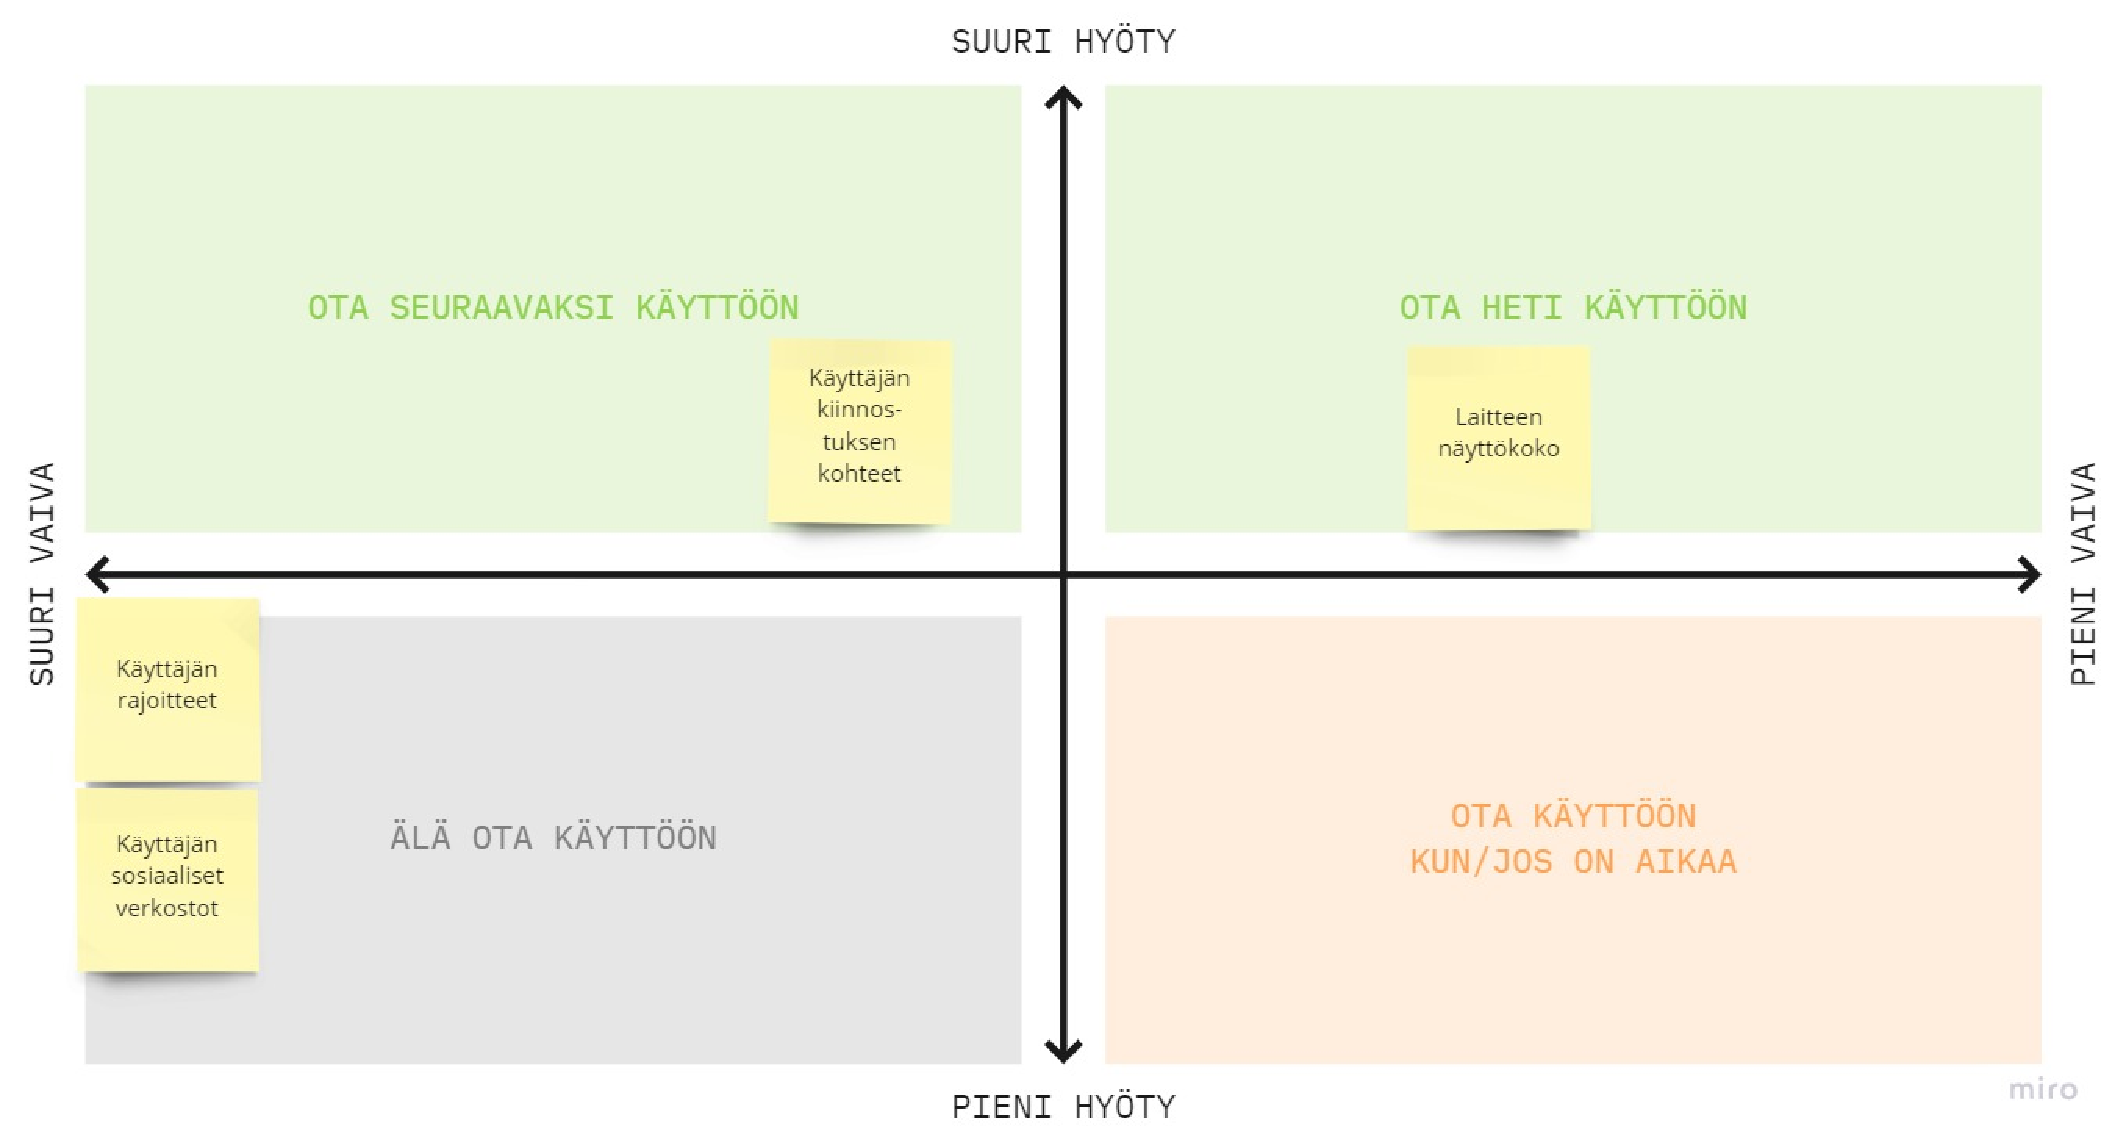
\includegraphics[width=\textwidth]{images/layout-priorization.pdf}
    \caption{Tärkeimmät sisällön asettelun personointimenetelmät.~\label{fig:layout-priorization}}
\end{figure}

\subsubsection{Typografia}

Typografian personointimenetelmiä tarkasteltiin tarkemmin
luvussa~\ref{typography-personalization}.

{\tiny\tabcolsep=3pt
\begin{longtable}{p{2.5cm}|p{6cm}|p{0.5cm}p{0.5cm}p{0.5cm}|p{0.5cm}|p{0.5cm}p{0.5cm}p{0.5cm}|p{0.5cm}|}
    \caption{Typografian personoinnin näkökulmien pisteytys.\label{table:typography-personalization-comparison}}                                                                                                                                                                                                                                                                                                                                                                                                                                                                                                                               \\
    \multirow[t]{2}{*}{\textbf{Näkökulma}} & \multirow[t]{2}{*}{\textbf{Menetelmän kuvaus}}                                                                                                                                                                                                                & \multicolumn{4}{c|}{\textbf{Vaivattomuus}} & \multicolumn{4}{c|}{\textbf{Hyöty}}                                                                                                                                                                                                                                                  \\\cline{3-10}
                                           &                                                                                                                                                                                                                                                               & \vertical{\textbf{Toteutuksen helppous}}   & \vertical{\textbf{Monistettavuus}}  & \vertical{\textbf{Käyttö toimialalla}} & \vertical{\textbf{Yhteensä}} & \vertical{\textbf{Vaikutus käyttökokemukseen}~} & \vertical{\textbf{Kohdennuksen tarkkuus}} & \vertical{\textbf{Tulevaisuuden näkymät}} & \vertical{\textbf{Yhteensä}} \\
    \midrule
    \textbf{Käyttäjä}                                                                                                                                                                                                                                                                                                                                                                                                                                                                                                                                                                                                                          \\
    \midrule
    Rajoitteet                             & Rello ym.~\cite{10.1145/2207016.2207048} tutkivat web-typografian personointia lukihäiriön näkökulmasta. Hyöty typografian personoinnista lukihäiriöstä kärsiville on merkittävä. Tieto rajoitteista kerättävä käyttäjältä erikseen.                          & 1                                          & 0                                   & 0                                      & 1                            & 10                                              & 1                                         & 1                                         & 12                           \\
    \midrule
    Ikä                                    & Hussain ym.~\cite{hussain_sohaib_ahmed_qasim_khan_2011} löysivät eroja eri ikäryhmien typografiamieltymyksissä. Käytännön hyöty on vielä epäselvä.                                                                                                            & 1                                          & 1                                   & 0                                      & 2                            & 1                                               & 1                                         & 0                                         & 2                            \\
    \midrule
    Sukupuoli                              & Vaikutusta ei ole tutkittu.                                                                                                                                                                                                                                   & 0                                          & 1                                   & 0                                      & 1                            & 0                                               & 0                                         & 0                                         & 0                            \\
    \midrule
    Kulttuuritausta                        & Reinecke ym.~\cite{10.1145/2556288.2557052} eivät ota tutkimuksessaan suoraan kantaa typografian personoinnin hyötyihin, joten vaikutusta ei ole tutkittu. Eri kirjoitusjärjestelmät täytyy ottaa huomioon sisällön näkökulmasta.                             & 0                                          & 1                                   & 0                                      & 1                            & 0                                               & 1                                         & 0                                         & 1                            \\
    \midrule
    Koulutustausta                         & Vaikutusta ei ole tutkittu. Tieto koulutustaustasta saatavilla julkishallinnon tietokannoista tai käyttäjältä erikseen pyydettynä.                                                                                                                            & 0                                          & 0                                   & 0                                      & 0                            & 0                                               & 1                                         & 0                                         & 1                            \\
    \midrule
    Kiinnostuksen kohteet                  & Vaikutusta ei ole tutkittu. Kiinnostuksen kohteet pääteltävissä käyttäytymisestä sivustolla.                                                                                                                                                                  & 0                                          & 1                                   & 0                                      & 1                            & 0                                               & 10                                        & 0                                         & 10                           \\
    \midrule
    Mieliala                               & Choi ja Aizawa~\cite{choi_aizawa_2018} löysivät, että typografian muuttaminen mielialan mukaan tekee viestittelystä eläväisempää. Ei selkeää keinoa kerätä tietoa.                                                                                            & 1                                          & 0                                   & 0                                      & 1                            & 10                                              & 1                                         & 0                                         & 11                           \\
    \midrule
    Sosiaaliset verkostot                  & Vaikutusta ei ole tutkittu. Tieto saatavilla suuntaa antavasti sosiaalisen median kautta käyttäjän suostumuksella.                                                                                                                                            & 0                                          & 0                                   & 0                                      & 0                            & 0                                               & 10                                        & 0                                         & 10                           \\
    \midrule
    \textbf{Käyttöympäristö}                                                                                                                                                                                                                                                                                                                                                                                                                                                                                                                                                                                                                   \\
    \midrule
    Laitteen näyttökoko                    & Darroch ym.~\cite{10.1007/11555261_23} löysivät yhteyden laitteen näyttökoon ja kirjasinkoon välillä. Kirjasinkoko mobiililaitteilla huomioidaan osana responsiivista web-suunnittelua.                                                                       & 10                                         & 0                                   & 10                                     & 20                           & 10                                              & 0                                         & 1                                         & 11                           \\
    \midrule
    Laitteen suorituskyky                  & Vaikutusta ei ole tutkittu.                                                                                                                                                                                                                                   & 0                                          & 1                                   & 0                                      & 1                            & 0                                               & 0                                         & 0                                         & 0                            \\
    \midrule
    Verkkoyhteyden laatu                   & Vaikutusta ei ole tutkittu, mutta hyöty on ilmeinen. Viime vuosina toimialalla on kehitetty ratkaisuja kuten esilataus~\cite{grigorik_2020} kirjasintyyppien latausajan minimoiseksi.                                                                         & 10                                         & 10                                  & 10                                     & 30                           & 10                                              & 0                                         & 10                                        & 20                           \\
    \midrule
    Sijainti                               & Vaikutusta ei ole tutkittu. Tieto saatavilla selainrajapintojen kautta käyttäjän suostumuksella.                                                                                                                                                              & 0                                          & 1                                   & 0                                      & 1                            & 0                                               & 1                                         & 0                                         & 1                            \\
    \midrule
    Aika                                   & Vaikutusta ei ole tutkittu.                                                                                                                                                                                                                                   & 0                                          & 1                                   & 0                                      & 1                            & 0                                               & 0                                         & 0                                         & 0                            \\
    \midrule
    Kirkkaus                               & Vaikutusta ei ole tutkittu, mutta hyöty vaikuttaa selkeältä. Tekstin kontrastin parantaminen kirkkaassa auringonvalossa esimerkiksi kirjasinkokoa suurentamalla on selkeä sovelluskohde. Tieto saatavilla selainrajapintojen kautta käyttäjän suostumuksella. & 0                                          & 1                                   & 0                                      & 1                            & 10                                              & 1                                         & 0                                         & 11                           \\
    \midrule
    Äänekkyys                              & Vaikutusta ei ole tutkittu. Tieto saatavilla selainrajapintojen kautta käyttäjän suostumuksella.                                                                                                                                                              & 0                                          & 1                                   & 0                                      & 1                            & 0                                               & 0                                         & 0                                         & 0                            \\
    \midrule
    Lämpötila ja sää                       & Vaikutusta ei ole tutkittu. Käyttäjän suostumuksella sijaintietoa voidaan käyttää säätietojen hakemiseen kolmannen osapuolen rajapinnasta.                                                                                                                    & 0                                          & 1                                   & 0                                      & 1                            & 0                                               & 0                                         & 0                                         & 0                            \\
    \midrule
    Liike                                  & Vaikutusta ei ole tutkittu, mutta ympäristön kirkkauden tapaan myös liikkeen tapauksessa tekstin kontrastin kasvattaminen parantaa luettavuutta. Tieto saatavilla selainrajapintojen kautta käyttäjän suostumuksella.                                         & 0                                          & 1                                   & 0                                      & 1                            & 10                                              & 1                                         & 0                                         & 11                           \\
\end{longtable}
}

Typografian personoinnin näkökulmat on pisteytetty
taulukkoon~\ref{table:typography-personalization-comparison}. Typografian
personointimenetelmien vertailussa korostuu sisällön asettelun tapaan
responsiivinen web-suunnittelu. Tekstin tulee olla luettavaa kaikilla
laitteilla, ja siksi esimerkiksi kirjasinkoon suurentaminen mobiililaitteilla on
erittäin hyödyllistä. Lisäksi tekstin luettavuuteen vaikuttavat tekijät, kuten
ympäristön kirkkaus, ja laitteen liike, kuten tärinä, nousevat hyödyllisiksi. Ne
eivät kuitenkaan tällä hetkellä ole helposti personoitavissa. Käyttäjälle
personoitava typografia ei nouse vertailussa kovin hyödylliseksi, vaan
tärkeimmät menetelmät painottuvat käyttöympäristön näkökulmien puolelle.
Tärkeimmät typografian personointimenetelmät on merkitty
kuvaan~\ref{fig:typography-priorization}.

\begin{figure}[h]
    \centering
    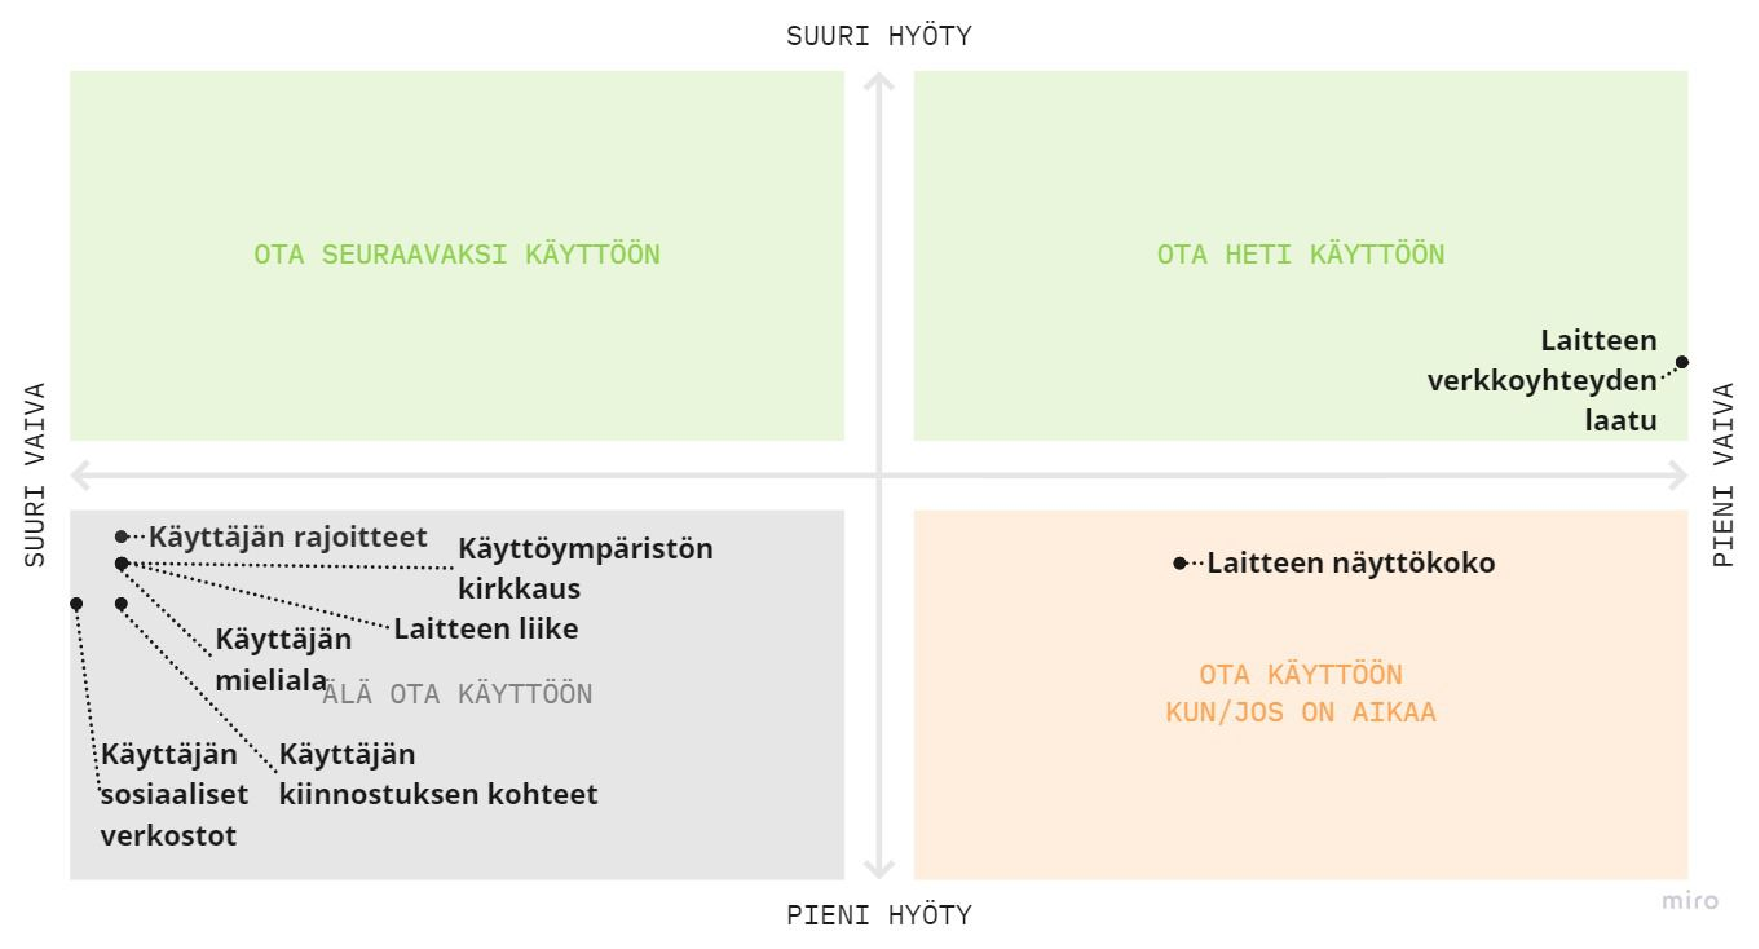
\includegraphics[width=\textwidth]{images/typography-priorization.pdf}
    \caption{Tärkeimmät typografian personointimenetelmät.~\label{fig:typography-priorization}}
\end{figure}

\subsubsection{Värit}

Värien personointimenetelmiä tarkasteltiin tarkemmin
luvussa~\ref{color-personalization}.

{\tiny\tabcolsep=3pt
\begin{longtable}{p{2.5cm}|p{6cm}|p{0.5cm}p{0.5cm}p{0.5cm}|p{0.5cm}|p{0.5cm}p{0.5cm}p{0.5cm}|p{0.5cm}|}
    \caption{Värien personoinnin näkökulmien pisteytys.\label{table:color-personalization-comparison}}                                                                                                                                                                                                                                                                                                                                                                                                                                                                                                                                                                                                \\
    \multirow[t]{2}{*}{\textbf{Näkökulma}} & \multirow[t]{2}{*}{\textbf{Menetelmän kuvaus}}                                                                                                                                                                                                                                                                       & \multicolumn{4}{c|}{\textbf{Vaivattomuus}} & \multicolumn{4}{c|}{\textbf{Hyöty}}                                                                                                                                                                                                                                                  \\\cline{3-10}
                                           &                                                                                                                                                                                                                                                                                                                      & \vertical{\textbf{Toteutuksen helppous}}   & \vertical{\textbf{Monistettavuus}}  & \vertical{\textbf{Käyttö toimialalla}} & \vertical{\textbf{Yhteensä}} & \vertical{\textbf{Vaikutus käyttökokemukseen}~} & \vertical{\textbf{Kohdennuksen tarkkuus}} & \vertical{\textbf{Tulevaisuuden näkymät}} & \vertical{\textbf{Yhteensä}} \\
    \midrule
    \textbf{Käyttäjä}                                                                                                                                                                                                                                                                                                                                                                                                                                                                                                                                                                                                                                                                                 \\
    \midrule
    Rajoitteet                             & Väripaletin personointi värisokeille kävijöille olisi hyödyllistä varsinkin graafisten sisältöjen ymmärtämisessä. Jefferson ja Harvey kehittivät menetelmän, jolla sivuston väripaletin voi automaattisesti korjata värisokeille.~\cite{10.1145/1168987.1168996}. Tieto rajoitteista kerättävä käyttäjältä erikseen. & 1                                          & 0                                   & 0                                      & 1                            & 10                                              & 1                                         & 1                                         & 12                           \\
    \midrule
    Ikä                                    & Reinecke ym.~\cite{10.1145/2556288.2557052} löysivät, että ikä vaikuttaa miellyttäväksi koettuihin väreihin. Käytännön hyöty on vielä epäselvä.                                                                                                                                                                      & 1                                          & 1                                   & 0                                      & 2                            & 1                                               & 1                                         & 0                                         & 2                            \\
    \midrule
    Sukupuoli                              & Reinecke ym.~\cite{10.1145/2556288.2557052} löysivät, että sukupuoli vaikuttaa miellyttäväksi koettuihin väreihin. Käytännön hyöty on vielä epäselvä.                                                                                                                                                                & 1                                          & 1                                   & 0                                      & 2                            & 1                                               & 1                                         & 0                                         & 2                            \\
    \midrule
    Kulttuuritausta                        & Reinecke ym.~\cite{10.1145/2556288.2557052} löysivät, että kulttuuritausta vaikuttaa miellyttäväksi koettuihin väreihin. Käytännön hyöty on vielä epäselvä.                                                                                                                                                          & 1                                          & 1                                   & 0                                      & 2                            & 1                                               & 1                                         & 0                                         & 2                            \\
    \midrule
    Koulutustausta                         & Vaikutusta ei ole tutkittu. Tieto koulutustaustasta saatavilla julkishallinnon tietokannoista tai käyttäjältä erikseen pyydettynä.                                                                                                                                                                                   & 0                                          & 1                                   & 0                                      & 1                            & 0                                               & 1                                         & 0                                         & 1                            \\
    \midrule
    Kiinnostuksen kohteet                  & Vaikutusta ei ole tutkittu, mutta Salesforcen Einstein Designer -konsepti~\cite{salesforce-einstein-designer} personoi myös värejä sivustokäyttäytymisen pohjalta.                                                                                                                                                                                       & 0                                          & 10                                  & 1                                      & 11                           & 1                                               & 10                                        & 10                                        & 21                           \\
    \midrule
    Mieliala                               & Vaikutusta ei ole tutkittu. Ei selkeää keinoa kerätä tietoa.                                                                                                                                                                                                                                                         & 0                                          & 0                                   & 0                                      & 0                            & 1                                               & 1                                         & 0                                         & 2                            \\
    \midrule
    Sosiaaliset verkostot                  & Vaikutusta ei ole tutkittu. Tieto saatavilla suuntaa antavasti sosiaalisen median kautta käyttäjän suostumuksella.                                                                                                                                                                                                   & 0                                          & 0                                   & 0                                      & 0                            & 0                                               & 10                                        & 0                                         & 10                           \\
    \midrule
    \textbf{Käyttöympäristö}                                                                                                                                                                                                                                                                                                                                                                                                                                                                                                                                                                                                                                                                          \\
    \midrule
    Laitteen näyttökoko                    & Vaikutusta ei ole tutkittu.                                                                                                                                                                                                                                                                                          & 0                                          & 1                                   & 0                                      & 1                            & 0                                               & 0                                         & 0                                         & 0                            \\
    \midrule
    Laitteen suorituskyky                  & Vaikutusta ei ole tutkittu.                                                                                                                                                                                                                                                                                          & 0                                          & 1                                   & 0                                      & 1                            & 0                                               & 0                                         & 0                                         & 0                            \\
    \midrule
    Verkkoyhteyden laatu                   & Vaikutusta ei ole tutkittu.                                                                                                                                                                                                                                                                                          & 0                                          & 1                                   & 0                                      & 1                            & 0                                               & 0                                         & 0                                         & 0                            \\
    \midrule
    Sijainti                               & Vaikutusta ei ole tutkittu. Tieto saatavilla selainrajapintojen kautta käyttäjän suostumuksella.                                                                                                                                                                                                                     & 0                                          & 1                                   & 0                                      & 1                            & 0                                               & 0                                         & 0                                         & 0                            \\
    \midrule
    Aika                                   & Vaikutusta ei ole tutkittu.                                                                                                                                                                                                                                                                                          & 0                                          & 1                                   & 0                                      & 1                            & 0                                               & 0                                         & 0                                         & 0                            \\
    \midrule
    Kirkkaus                               & Vaikutusta ei ole tutkittu, mutta hyöty vaikuttaa typografian tapaan selkeältä, joskaan ei yhtä merkittävältä värien toissijaisuuden vuoksi.                                                                                                                                                                         & 0                                          & 1                                   & 0                                      & 1                            & 1                                               & 1                                         & 0                                         & 2                            \\
    \midrule
    Äänekkyys                              & Vaikutusta ei ole tutkittu. Tieto saatavilla selainrajapintojen kautta käyttäjän suostumuksella.                                                                                                                                                                                                                     & 0                                          & 1                                   & 0                                      & 1                            & 0                                               & 0                                         & 0                                         & 0                            \\
    \midrule
    Lämpötila ja sää                       & Vaikutusta ei ole tutkittu. Käyttäjän suostumuksella sijaintietoa voidaan käyttää säätietojen hakemiseen kolmannen osapuolen rajapinnasta.                                                                                                                                                                           & 0                                          & 1                                   & 0                                      & 1                            & 0                                               & 0                                         & 0                                         & 0                            \\
    \midrule
    Liike                                  & Vaikutusta ei ole tutkittu. Tieto saatavilla selainrajapintojen kautta käyttäjän suostumuksella.                                                                                                                                                                                                                     & 0                                          & 1                                   & 0                                      & 1                            & 0                                               & 0                                         & 0                                         & 0                            \\
\end{longtable}
}

Värien personoinnin näkökulmat on pisteytetty
taulukkoon~\ref{table:color-personalization-comparison}. Värien personoinnissa
ei nouse esiin merkittävän hyödyllisiä personointikohteita. Reinecke
ym.~\cite{10.1145/2556288.2557052} tutkimus kyllä osoittaa yhteyden
värimieltymysten ja erinäisten ominaisuuksien, kuten iän ja sukupuolen välillä,
mutta käytännön tasolla menetelmät on hankala ottaa käyttöön sivustolla. Värien
osalta tärkeimmät personointimenetelmät ovat värisokeuden huomioiminen ja
käyttäjän kiinnostuksen kohteiden pohjalta tehtävä ulkoasun personointi, jota
muun muassa Salesforcen Einstein Designer
-konsepti~\cite{salesforce-einstein-designer} on demonstroinut. Tärkeimmät
värien personointimenetelmät on merkitty kuvaan~\ref{fig:color-priorization}.

\begin{figure}[h]
    \centering
    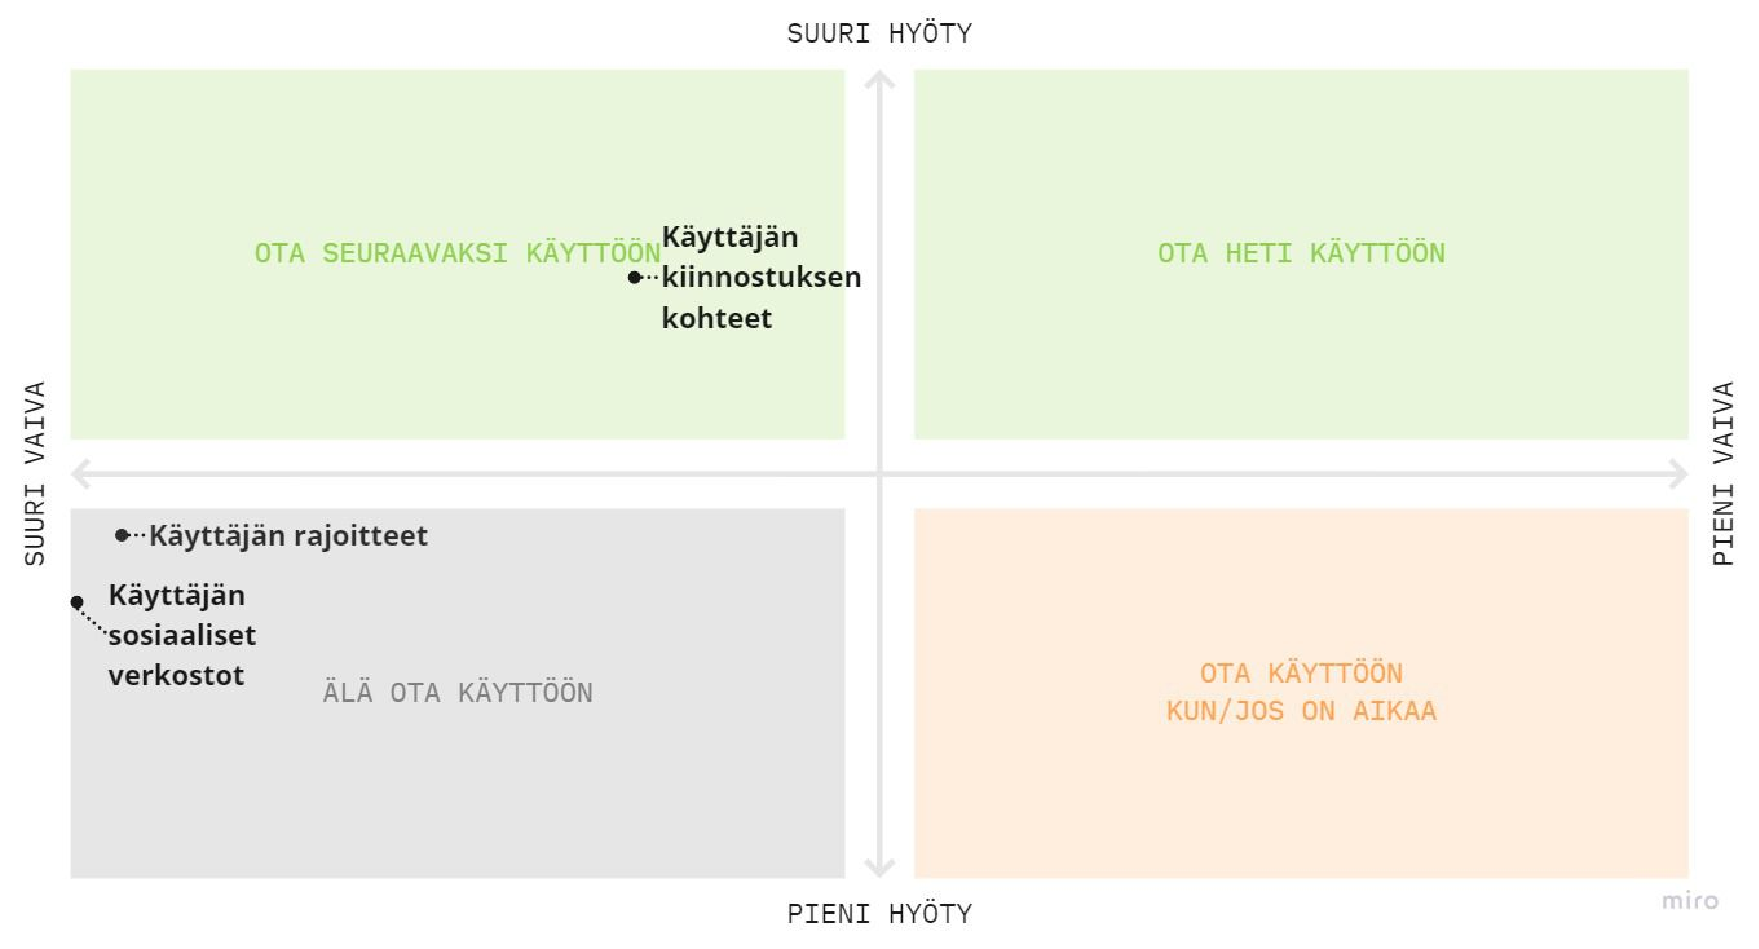
\includegraphics[width=\textwidth]{images/color-priorization.pdf}
    \caption{Tärkeimmät värien personointimenetelmät.~\label{fig:color-priorization}}
\end{figure}

\subsubsection{Kuvien muokkaus}

Kuvien muokkauksessa käytettäviä personointimenetelmiä tarkasteltiin tarkemmin
luvussa~\ref{images-personalization}.

{\tiny\tabcolsep=3pt
\begin{longtable}{p{2.5cm}|p{6cm}|p{0.5cm}p{0.5cm}p{0.5cm}|p{0.5cm}|p{0.5cm}p{0.5cm}p{0.5cm}|p{0.5cm}|}
    \caption{Kuvien muokkauksen personoinnin näkökulmien pisteytys.\label{table:images-personalization-comparison}}                                                                                                                                                                                                                                                                                                                                                                                                                                                                                                                                                                                                                                    \\
    \multirow[t]{2}{*}{\textbf{Näkökulma}} & \multirow[t]{2}{*}{\textbf{Menetelmän kuvaus}}                                                                                                                                                                                                                                                                                                                        & \multicolumn{4}{c|}{\textbf{Vaivattomuus}} & \multicolumn{4}{c|}{\textbf{Hyöty}}                                                                                                                                                                                                                                                  \\\cline{3-10}
                                           &                                                                                                                                                                                                                                                                                                                                                                       & \vertical{\textbf{Toteutuksen helppous}}   & \vertical{\textbf{Monistettavuus}}  & \vertical{\textbf{Käyttö toimialalla}} & \vertical{\textbf{Yhteensä}} & \vertical{\textbf{Vaikutus käyttökokemukseen}~} & \vertical{\textbf{Kohdennuksen tarkkuus}} & \vertical{\textbf{Tulevaisuuden näkymät}} & \vertical{\textbf{Yhteensä}} \\
    \midrule
    \textbf{Käyttäjä}                                                                                                                                                                                                                                                                                                                                                                                                                                                                                                                                                                                                                                                                                                                                  \\
    \midrule
    Rajoitteet                             & Vaikutusta ei ole suoraan tutkittu, mutta hyödyt samansuuntaisia kuin Jeffersonin ja Harveyn tutkimuksessa~\cite{10.1145/1168987.1168996}, jossa tarkasteltiin värien optimointia värisokeille. Hyödyt eivät ole yhtä merkittäviä, koska kuvia ei voida samaan tapaan vapaasti muokata kuin sivuston väripalettia. Tieto rajoitteista kerättävä käyttäjältä erikseen. & 0                                          & 0                                   & 0                                      & 0                            & 1                                               & 1                                         & 0                                         & 2                            \\
    \midrule
    Ikä                                    & Vaikutusta ei ole suoraan tutkittu, mutta kuvien kontrastin kasvattamisesta voisi olla hyötyä ikääntyneille.                                                                                                                                                                                                                                                          & 0                                          & 1                                   & 0                                      & 1                            & 1                                               & 1                                         & 0                                         & 2                            \\
    \midrule
    Sukupuoli                              & Vaikutusta ei ole tutkittu.                                                                                                                                                                                                                                                                                                                                           & 0                                          & 1                                   & 0                                      & 1                            & 0                                               & 1                                         & 0                                         & 1                            \\
    \midrule
    Kulttuuritausta                        & Vaikutusta ei ole tutkittu.                                                                                                                                                                                                                                                                                                                                           & 0                                          & 0                                   & 0                                      & 0                            & 0                                               & 1                                         & 0                                         & 1                            \\
    \midrule
    Koulutustausta                         & Vaikutusta ei ole tutkittu. Tieto koulutustaustasta saatavilla julkishallinnon tietokannoista tai käyttäjältä erikseen pyydettynä.                                                                                                                                                                                                                                    & 0                                          & 0                                   & 0                                      & 0                            & 0                                               & 1                                         & 0                                         & 1                            \\
    \midrule
    Kiinnostuksen kohteet                  & Kang ym.~\cite{5539850} löysivät, että käyttäjä suosii omien mieltymystensä mukaan muokattuja kuvia. Kim ym.~\cite{10.1007/978-3-030-58577-8_23} jatkokehittivät Kang ym.~menetelmää ja julkaisivat referenssitoteutuksensa. Mieltymykset täytyy kerätä erikseen käyttäjältä etukäteen.                                                                               & 10                                         & 0                                   & 0                                      & 10                           & 10                                              & 10                                        & 1                                         & 21                           \\
    \midrule
    Mieliala                               & Vaikutusta ei ole tutkittu, mutta Kang ym.\cite{5539850} tulokset pätevät jos käyttäjän mieltymykset kerätään halutussa mielialassa.                                                                                                                                                                                                                                  & 0                                          & 0                                   & 0                                      & 0                            & 10                                              & 10                                        & 0                                         & 20                           \\
    \midrule
    Sosiaaliset verkostot                  & Vaikutusta ei ole tutkittu. Tieto saatavilla suuntaa antavasti sosiaalisen median kautta käyttäjän suostumuksella.                                                                                                                                                                                                                                                    & 0                                          & 0                                   & 0                                      & 0                            & 0                                               & 10                                        & 0                                         & 10                           \\
    \midrule
    \textbf{Käyttöympäristö}                                                                                                                                                                                                                                                                                                                                                                                                                                                                                                                                                                                                                                                                                                                           \\
    \midrule
    Laitteen näyttökoko                    & Kuvien älykäs rajaus eri näyttöko'oille on hyödyllistä. Kang ym.~\cite{5539850} pohtivat että tutkimusta ja vaikutusten arviointia voisi jatkaa myös rajauksen optimoinnin osalta, mutta tällä haavaa vaikutusta ei ole vielä tutkittu. Toimialalla on useita ratkaisuja älykkääseen rajaukseen (engl.~\textit{smart cropping}).                                      & 10                                         & 10                                  & 10                                     & 30                           & 10                                              & 1                                         & 10                                        & 21                           \\
    \midrule
    Laitteen suorituskyky                  & Vaikutusta ei ole tutkittu.                                                                                                                                                                                                                                                                                                                                           & 0                                          & 0                                   & 0                                      & 0                            & 0                                               & 0                                         & 0                                         & 0                            \\
    \midrule
    Verkkoyhteyden laatu                   & Vaikutusta ei ole tutkittu, mutta viime vuosina on kehitetty useita kuvaformaatteja, kuten WebP ja AVIF, jotka pakkaavat kuvan tehokkaamin kuin perinteiset JPEG tai PNG, ja vievät siten vähemmän tilaa. Kuvaformaatin personointi verkkoyhteyden laadun perusteella tuo siis merkittäviä hyötyjä.                                                                   & 10                                         & 10                                  & 10                                     & 30                           & 10                                              & 0                                         & 10                                        & 20                           \\
    \midrule
    Sijainti                               & Vaikutusta ei ole tutkittu. Tieto saatavilla selainrajapintojen kautta käyttäjän suostumuksella.                                                                                                                                                                                                                                                                      & 0                                          & 1                                   & 0                                      & 1                            & 0                                               & 0                                         & 0                                         & 0                            \\
    \midrule
    Aika                                   & Vaikutusta ei ole tutkittu.                                                                                                                                                                                                                                                                                                                                           & 0                                          & 1                                   & 0                                      & 1                            & 0                                               & 0                                         & 0                                         & 0                            \\
    \midrule
    Kirkkaus                               & Vaikutusta ei ole tutkittu, mutta hyöty vaikuttaa typografian tapaan selkeältä. Kirkkaassa auringonpaisteessa kuvan kontrastia voidaan kasvattaa. Pimeässä kuva voidaan esittää yötilan kaltaisesti.                                                                                                                                                                  & 0                                          & 1                                   & 0                                      & 1                            & 10                                              & 1                                         & 0                                         & 11                           \\
    \midrule
    Äänekkyys                              & Vaikutusta ei ole tutkittu. Tieto saatavilla selainrajapintojen kautta käyttäjän suostumuksella.                                                                                                                                                                                                                                                                      & 0                                          & 1                                   & 0                                      & 1                            & 0                                               & 0                                         & 0                                         & 0                            \\
    \midrule
    Lämpötila ja sää                       & Vaikutusta ei ole tutkittu. Tieto saatavilla selainrajapintojen kautta käyttäjän suostumuksella.                                                                                                                                                                                                                                                                      & 0                                          & 1                                   & 0                                      & 1                            & 0                                               & 0                                         & 0                                         & 0                            \\
    \midrule
    Liike                                  & Vaikutusta ei ole tutkittu. Tieto saatavilla selainrajapintojen kautta käyttäjän suostumuksella.                                                                                                                                                                                                                                                                      & 0                                          & 1                                   & 0                                      & 1                            & 0                                               & 0                                         & 0                                         & 0                            \\
\end{longtable}
}

Kuvien muokkauksen personoinnin näkökulmat on pisteytetty
taulukkoon~\ref{table:images-personalization-comparison}. Kuvien muokkaus nousee
personointinäkökulmien ja -menetelmien vertailussa sisällön asettelun rinnalle
arvioidussa tärkeydessä. Kuvien muokkauksen personoinnissa korostuu sisällön
asettelun tapaan responsiivinen web-suunnittelu, eli esimerkiksi kuvaformaattien
optimointi heikolle verkkoyhteydelle ja kuvien älykäs rajaus mobiililaitteille.
Myös käyttäjän rajoitusten, kuten huonon näön tai värisokeuden huomioiminen
nousee tärkeäksi personointikeinoksi. Myös Kang ym.~\cite{5539850} tutkimuksessa
kuvattu käyttäjän mieltymysten mukainen kuvien muokkaus vaikuttaa lupaavalta.
Tärkeimmät kuvien personointimenetelmät on merkitty
kuvaan~\ref{fig:images-priorization}.

\begin{figure}[h]
    \centering
    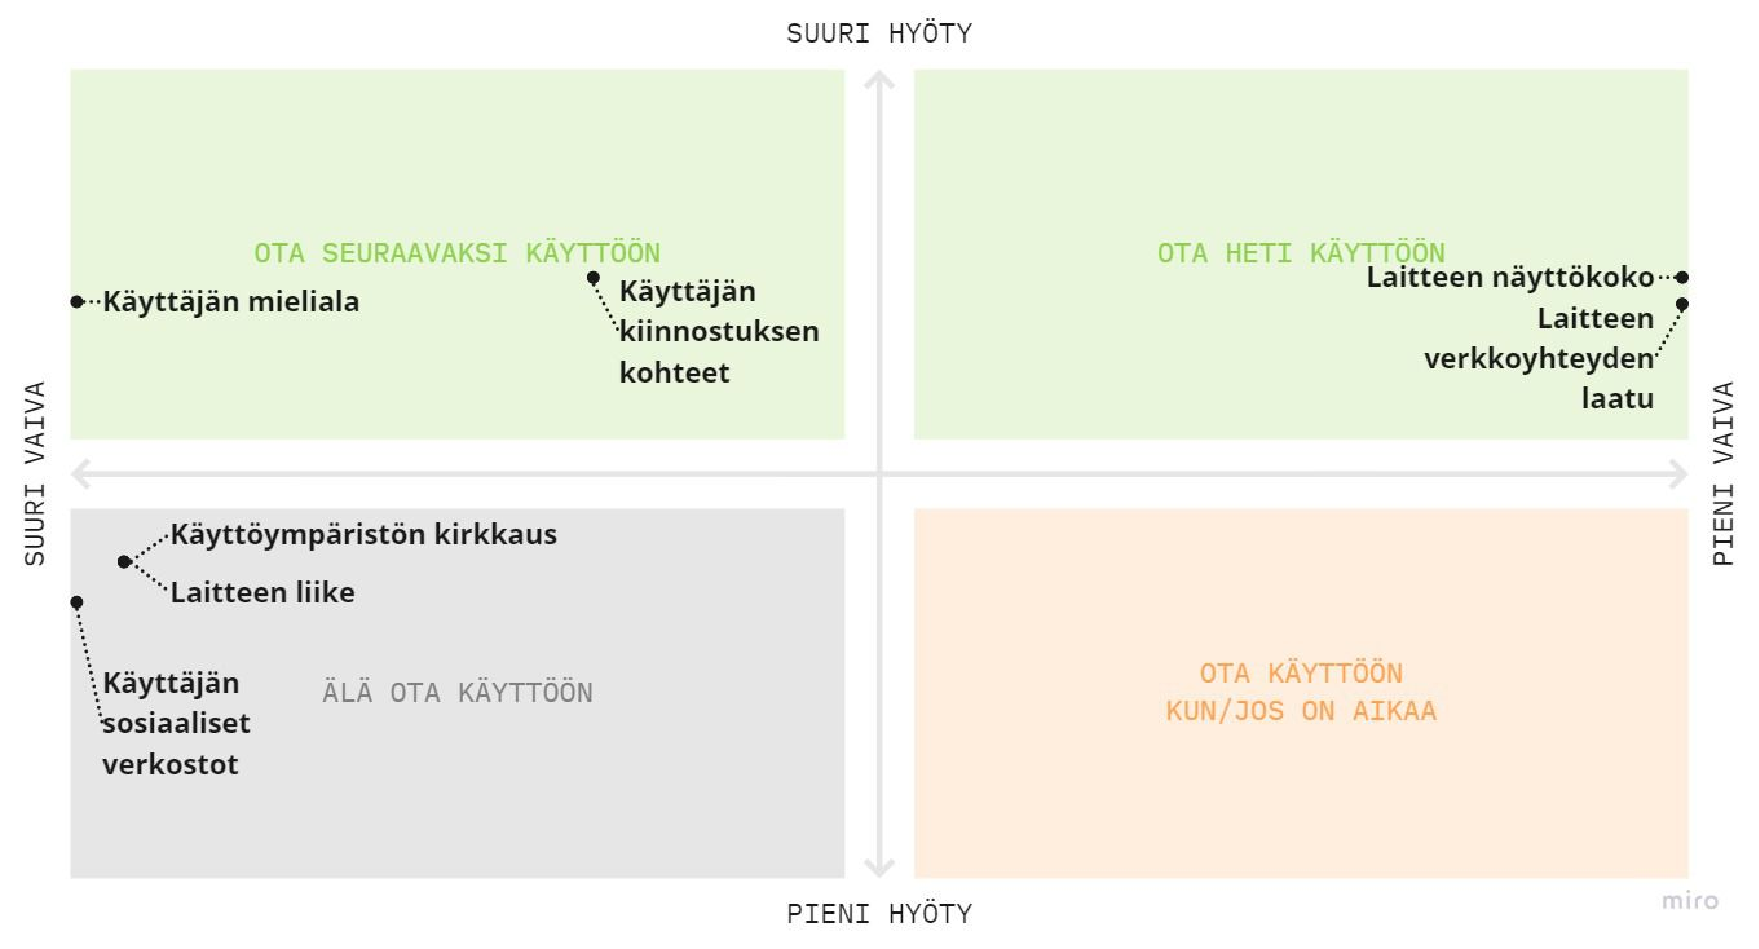
\includegraphics[width=\textwidth]{images/images-priorization.pdf}
    \caption{Tärkeimmät kuvien muokkauksen personointimenetelmät.~\label{fig:images-priorization}}
\end{figure}

\subsection{Yhteenveto}

Tässä luvussa vertailtiin personoinnin eri näkökulmia pisteyttämällä ne luvun
alussa esitellyn kriteeristön perusteella. Pisteytys tehtiin erikseen jokaiselle
työssä tarkasteltavista sivuston ulkoasun osa-alueista, joita ovat sisällön
asettelu, typografia, värit ja kuvien muokkaus. Pisteytetyt näkökulmat koottiin
osa-aluekohtaiseen priorisointikaavioon, josta näkee helposti mitä
personoinnin näkökulmia ja menetelmiä kannattaa palveluntarjoajana lähteä
edistämään ensimmäisenä.

Priorisointikaavioiden parhaassa, eli hyödyllisimmässä ja vaivattomimmassa,
kulmassa korostuvat ne personoinnin näkökulmat, jotka ovat jo vakiintuneet
toimialalle. Tällainen näkökulma on esimerkiksi sisällön asettelun personointi
laitteen näyttökoon perusteella, johon löytyy valmis menetelmä, eli
responsiivinen web-suunnittelu. Typografian ja kuvien muokkauksen personointi
verkkoyhteyden laadun perusteella nousi myös kaavioiden parhaaseen kulmaan
toimialaratkaisujen, kuten fonttien esilatauksen ja uusien kuvaformaattien,
siivittämänä.

Kuvien muokkauksen personointi korostuu hyödyllisyyden osalta, sillä jopa neljä
näkökulmaa nousi osa-alueen osalta esiin sellaisina, joita kannattaa edistää.
Myös sisällön asettelun personoinnin osalta löytyi useampi hyödyllinen
näkökulma. Sekä värien että typografian personoinnin osalta hyödyllisiä
näkökulmia löytyi vain yksi. Sen sijaan molemmille näistä osa-alueista löytyi
useampi näkökulma, jotka saivat jonkin verran pisteitä hyödyllisyydestä, mutta
jotka eivät saaneet lähes yhtään pisteitä vaivattomuudesta. Näkökulmia, kuten
typografian personointi laitteen liikkuessa ja värien personointi käyttäjän
sosiaalisten verkostojen perusteella, ei kannata edistää vaikka niiden
hyödyllisyydestä onkin näyttöä.

Yksi työn tavoitteista oli löytää vertailun avulla personointimenetelmät, joista
saa suurimman hyödyn pienimmällä vaivalla. Tässä luvussa esiteltyjen
priorisointikaavioiden avulla palveluntarjoaja voi helposti vertailla eri
personoinnin näkökulmia ja pohtia, mitä niistä kannattaisi lähteä edistämään
web-sivustollaan.

\clearpage
\section{Yhteenveto}

Tässä työssä tarkasteltiin web-sivuston ulkoasun personointimenetelmiä
erinäisistä käyttäjä- ja ympäristölähtöisistä näkökulmista.
Personointimenetelmiä esiteltiin sivuston eri osa-alueiden, kuten asettelun,
värien ja typografian kautta. Tarkasteltuja käyttäjälähtöisiä näkökulmia oli
muun muassa rajoitteet, kuten näkö- ja liikuntavammat, ikä ja kulttuuritausta.
Tarkasteltuja ympäristölähtöisiä näkökulmia olivat muun muassa laitteen
näyttökoko, suorituskyky ja käyttöympäristön ominaisuudet, kuten valoisuus.

Työ oli rajattu sivuston ulkoasun personointiin. Sivuston ulkoasun suunnittelu
ja toteutus ovat edelleen pitkälti manuaalista työtä. Sivustoa on hankala
suunnitella jokaiselle käyttäjälle sopivaksi, koska käyttäjillä on eri
mieltymyksiä ulkoasun suhteen muun muassa kulttuuritaustasta riippuen. Työssä
selvitettiin voisiko tätä ongelmaa ratkaista sivuston ulkoasun
personointimenetelmillä, jotka perustuvat matemaattiseen optimointiin ja
käyttöliittymäsuunnittelun heuristiikkoihin. Sisällön personointi jätettiin työn
ulkopuolelle, sillä sen sisällyttäminen olisi kasvattanut työn rajausta liian
suureksi.

Työ vertaili havaittuja personointimenetelmiä pisteyttämällä ne vaivattomuuden
ja arvioidun hyödyn saralla. Molempien akselien pisteytykseen kehitettiin
kriteeristö, jonka pisteytysasteikko on eksponentiaalinen erojen
selkeyttämiseksi. Pisteytyksessä kaikkia työhön valittuja personoinnin
näkökulmia tarkasteltiin erikseen jokaisen sivuston osa-alueen kannalta. Pisteet
kuvattiin priorisointikaavioon, josta näkee selkeästi mitkä menetelmistä
kannattaa ottaa heti käyttöön, mitkä kannattaa ottaa seuraavaksi käyttöön, mitä
menetelmiä kannattaa harkita, ja mitä ei kannata ottaa käyttöön.

Työssä löydettiin, että suurin osa tarkastelluista menetelmistä on sellaisia,
joita ei kannata ottaa käyttöön. Hyödyllisiä ja vaivattomia
personointimenetelmiä, eli menetelmiä, jotka kannattaa ottaa heti käyttöön, ei
ollut montaa, ja niissä korostui vakiintuneisuus toimialalla. Tärkein tällainen
menetelmä on sisällön asettelun personointi laitteen näyttökoon perusteella, eli
responsiivinen web-suunnittelu. Hyödyllisissä mutta vähemmän vaivattomaksi
havaituissa menetelmissä korostui teknisesti vaativammat menetelmät. Tällaisia
menetelmiä ovat muun muassa sisällön asettelun personointi käyttäjän
kiinnostuksen kohteiden mukaan ja responsiivisen web-suunnittelun automaatio
laskennallisilla menetelmillä. Moni menetelmä havaittiin hyödylliseksi, mutta
toteutus vaatii suuren vaivan, esimerkiksi uuden teknologian kehityksen.
Tällaiseksi menetelmäksi havaittiin muun muassa värien personointi käyttäjän
rajoitteiden, kuten näkövamman perusteella.

Web-sivuston ulkoasun personointiin on siis muutama selkeä, mutta suurilta osin
jo toimialalle vakiintunut menetelmä. Ulkoasun personoinnin automaatioon ei
tällä hetkellä löydy toimialaratkaisuja, jotka olisi mahdollista ottaa käyttöön
pienellä vaivalla. Personointiin ja sivuston ulkoasun suunnittelun ja
toteutuksen automaatioon kohdistuu kuitenkin vireää tutkimusta, mikä
toivottavasti näkyy lähiaikoina myös käytännön ratkaisuina toimialalla.

\clearpage

\thesisbibliography{}
\printbibliography{}

\end{document}
